% Paper 1a. Every number in this file is a macro from tables/numbers.tex, and every table
% and figure is generated: `make all` regenerates them from the tracked results snapshot
% before compiling. Do not type a measured value into this file.
%
% The one exception is Table \ref{tab:direction}, which carries no measurement: it states
% the direction of translation of each corpus, read off that corpus's own documentation,
% and the sign that direction puts on the ratio. It is written out here because there is
% nothing in results.json for a script to read it from.
\documentclass[11pt]{article}

% Build mode. `mode.tex` loads acl.sty with either [final] or [review] and sets the
% \iffinalmode switch this file uses to gate the acknowledgements and the repository URL.
% It is tracked in final mode; `make review` rewrites it, builds, and restores it.
% Build mode for paper/1a. `make pdf` and `make arxiv` build with this file as tracked;
% `make review` overwrites it, builds main_review.pdf, and restores it. The tracked
% default is final, so a plain `tectonic main.tex` produces the de-anonymised paper.
%
% \finalmodetrue  -> author block shown, acknowledgements printed, repository URL given.
% \finalmodefalse -> anonymised author block, line numbers, no acknowledgements, no URL.
\newif\iffinalmode
\finalmodetrue
\usepackage[final]{acl}


\usepackage{times}
\usepackage{latexsym}
\usepackage{booktabs}
\usepackage{graphicx}
\usepackage{amsmath}
\usepackage{microtype}
\usepackage{xcolor}
\usepackage[T1]{fontenc}
\usepackage[utf8]{inputenc}
% \FloatBarrier before the bibliography, so that no body float is deferred into the
% references. ARR desk checks flag that, and it happened to two tables and a figure here.
\usepackage{placeins}

% Float placement. Section 5.5 cites two full-width tables and a figure inside two
% paragraphs, and LaTeX's defaults let at most two floats onto a page and reserve a fifth
% of it for text, which pushed the figure three pages past its first reference. These are
% the usual relaxations; nothing here forces a float anywhere.
\setcounter{topnumber}{3}
\setcounter{bottomnumber}{2}
\setcounter{totalnumber}{4}
\renewcommand{\topfraction}{0.92}
\renewcommand{\bottomfraction}{0.9}
\renewcommand{\textfraction}{0.07}
\renewcommand{\floatpagefraction}{0.72}

% Generated by scripts/paper_tables.py from results/. Do not edit.
% Every number in the manuscript's prose is one of these macros.
\newcommand{\numFloresSents}{1,012}
\newcommand{\numSamayikTest}{2,417}
\newcommand{\numSamayikOod}{4,047}
\newcommand{\numItihasaTest}{11,721}
\newcommand{\numBootstrap}{1000}
\newcommand{\numBootstrapSeed}{0}
\newcommand{\numCiLevel}{95}
\newcommand{\numSaWords}{16,975}
\newcommand{\numEnWords}{21,901}
\newcommand{\numHiWords}{25,643}
\newcommand{\numParitySaEnLo}{1.774}
\newcommand{\numParitySaEnHi}{2.187}
\newcommand{\numParitySaEnGptTwo}{7.857}
\newcommand{\numParitySaHiLo}{1.060}
\newcommand{\numParitySaHiHi}{1.353}
\newcommand{\numParitySaHiLargeLo}{1.325}
\newcommand{\numParitySaHiLargeHi}{1.353}
\newcommand{\numFertSaLo}{3.11}
\newcommand{\numFertSaHi}{3.88}
\newcommand{\numFertSaGptTwo}{12.49}
\newcommand{\numFertSaGptTwoSlpOne}{3.97}
\newcommand{\numFertRatioSaEnLo}{2.31}
\newcommand{\numFertRatioSaEnHi}{8.38}
\newcommand{\numFertRatioSaHiLo}{1.60}
\newcommand{\numFertRatioSaHiHi}{1.74}
\newcommand{\numCompSaOrigLo}{1.63}
\newcommand{\numCompSaOrigHi}{7.21}
\newcommand{\numCompEnLo}{4.87}
\newcommand{\numCompEnHi}{4.92}
\newcommand{\numCompSaSlpLo}{2.05}
\newcommand{\numCompSaSlpHi}{2.38}
\newcommand{\numPreregFertLo}{5}
\newcommand{\numPreregFertHi}{12}
\newcommand{\numPreregHindiFertLo}{2}
\newcommand{\numPreregHindiFertHi}{4}
\newcommand{\numPreregParityThreshold}{1.5}
\newcommand{\numDeployedLo}{1.831}
\newcommand{\numDeployedHi}{2.899}
\newcommand{\numDeployedSamayikOTwoHundredK}{1.835}
\newcommand{\numDeployedSamayikOTwoHundredKCi}{[1.813, 1.858]}
\newcommand{\numTppBpeSixtyFourDeployed}{0.887}
\newcommand{\numTppBpeSixtyFourDeployedCi}{[0.875, 0.899]}
\newcommand{\numTppControlledBest}{1.035}
\newcommand{\numTppControlledBestCi}{[1.021, 1.049]}
\newcommand{\numTppControlledBpeThirtyTwo}{1.084}
\newcommand{\numTppControlledSamayikLo}{1.030}
\newcommand{\numTppControlledSamayikHi}{1.142}
\newcommand{\numTppControlledOodLo}{1.055}
\newcommand{\numTppControlledOodHi}{1.163}
\newcommand{\numTppControlledFloresLo}{1.131}
\newcommand{\numTppControlledFloresHi}{1.219}
\newcommand{\numTppControlledItihasaLo}{0.597}
\newcommand{\numTppControlledItihasaHi}{0.658}
\newcommand{\numTppControlledItihasaAllLo}{0.555}
\newcommand{\numTppControlledItihasaAllHi}{0.658}
\newcommand{\numTppControlledHugeOodLo}{1.015}
\newcommand{\numTppControlledHugeOodHi}{1.145}
\newcommand{\numControlledPairs}{4}
\newcommand{\numControlledPairsAll}{12}
\newcommand{\numControlledPairsSmall}{8}
\newcommand{\numControlledPairsHuge}{4}
\newcommand{\numBmLines}{78,624}
\newcommand{\numBmLinePct}{67.7}
\newcommand{\numBytesSanskritTrain}{11.21}
\newcommand{\numBytesEnglishTrain}{16.55}
\newcommand{\numBytesEnglishBmTrain}{11.21}
\newcommand{\numBytesEnglishExcessPct}{48}
\newcommand{\numBmMoveCount}{24}
\newcommand{\numBmMaxMove}{0.025}
\newcommand{\numBmMedianMove}{0.008}
\newcommand{\numBmDownwardCount}{23}
\newcommand{\numBmVerdictChanges}{0}
\newcommand{\numVocabHuge}{128,000}
\newcommand{\numTppBpeHugeSamayik}{0.983}
\newcommand{\numTppBpeHugeSamayikCi}{[0.971, 0.997]}
\newcommand{\numTppBpeHugeSamayikBm}{0.978}
\newcommand{\numTppBpeHugeSamayikBmCi}{[0.965, 0.991]}
\newcommand{\numTppBpeHugeOod}{1.025}
\newcommand{\numTppBpeHugeOodCi}{[1.013, 1.037]}
\newcommand{\numTppBpeHugeOodBlockCi}{[0.999, 1.050]}
\newcommand{\numTppBpeHugeFlores}{1.116}
\newcommand{\numBpeMonotoneSequences}{7}
\newcommand{\numBpeSequencesTotal}{8}
\newcommand{\numBpeFloresStepGap}{0.001}
\newcommand{\numUnigramBmPieces}{50,659}
\newcommand{\numUnigramHugePieces}{62,896}
\newcommand{\numCharRatioSamayik}{1.028}
\newcommand{\numCharRatioItihasa}{0.596}
\newcommand{\numCharRatioFactor}{1.725}
\newcommand{\numDensityRatioSamayikLo}{1.002}
\newcommand{\numDensityRatioSamayikHi}{1.111}
\newcommand{\numDensityRatioItihasaLo}{1.001}
\newcommand{\numDensityRatioItihasaHi}{1.104}
\newcommand{\numDensityRatioSamayikHugeLo}{0.951}
\newcommand{\numDensityRatioSamayikHugeHi}{0.956}
\newcommand{\numDensityPairGap}{0.032}
\newcommand{\numTSevenSamayik}{1.027}
\newcommand{\numTSevenItihasa}{0.595}
\newcommand{\numTSevenVocab}{256}
\newcommand{\numBlockLength}{50}
\newcommand{\numBlockRowsPerCorpus}{13}
\newcommand{\numBlockWidenItihasaLo}{2.4}
\newcommand{\numBlockWidenItihasaHi}{2.6}
\newcommand{\numBlockWidenFloresLo}{2.1}
\newcommand{\numBlockWidenFloresHi}{2.6}
\newcommand{\numBlockWidenOodLo}{1.8}
\newcommand{\numBlockWidenOodHi}{2.4}
\newcommand{\numBlockWidenSamayikLo}{0.9}
\newcommand{\numBlockWidenSamayikHi}{1.0}
\newcommand{\numBlockNarrowerSamayik}{11}
\newcommand{\numBlockItihasaMaxUpper}{0.667}
\newcommand{\numEnTokensOTwoHundredK}{39,339}
\newcommand{\numEnTokensEOneBpe}{33,702}
\newcommand{\numEnTokenSavingPct}{14.3}
\newcommand{\numUnigramSixtyFourPieces}{62,896}
\newcommand{\numUnigramSixtyFourShortfallPct}{1.7}
\newcommand{\numVocabMin}{50,257}
\newcommand{\numVocabMax}{262,145}
\newcommand{\numLargeVocabFloor}{200,019}
\newcommand{\numVocabSmall}{32,000}
\newcommand{\numVocabLarge}{64,000}
\newcommand{\numArmsDeployedGeneral}{4}
\newcommand{\numArmsDeployedIndic}{3}
\newcommand{\numTrainedArms}{6}
\newcommand{\numCheckedSentences}{19,197}
\newcommand{\numLeakedSentences}{0}
\newcommand{\numBytesPerDevanagariChar}{three}
\newcommand{\numSamayikTrain}{43,493}
\newcommand{\numItihasaTrain}{75,161}
\newcommand{\numTrainPairsTotal}{118,654}
\newcommand{\numRenyiAlpha}{2.5}
\newcommand{\numRenyiDeployedLo}{0.568}
\newcommand{\numRenyiDeployedHi}{0.581}
\newcommand{\numRenyiGptTwo}{0.270}
\newcommand{\numRenyiGptTwoSlpOne}{0.578}
\newcommand{\numRenyiDeployedSlpOneLo}{0.525}
\newcommand{\numRenyiDeployedSlpOneHi}{0.566}
\newcommand{\numRenyiBpeThirtyTwo}{0.615}
\newcommand{\numRenyiBpeSixtyFour}{0.589}
\newcommand{\numRenyiUnigramLo}{0.485}
\newcommand{\numRenyiUnigramHi}{0.493}
\newcommand{\numRenyiEnglishLo}{0.490}
\newcommand{\numRenyiEnglishHi}{0.508}
\newcommand{\numLengthSparseBelow}{30}
\newcommand{\numSamayikMeanEnWords}{12.5}
\newcommand{\numSamayikMeanSaWords}{9.6}
\newcommand{\numItihasaMeanEnWords}{30.7}
\newcommand{\numItihasaMeanSaWords}{11.2}
\newcommand{\numLengthGradientsFlipped}{16}
\newcommand{\numLengthGradientsTotal}{16}
\newcommand{\numLengthEnFirstBin}{1--8}
\newcommand{\numLengthEnFirstLo}{1.196}
\newcommand{\numLengthEnFirstHi}{1.304}
\newcommand{\numLengthEnLastBin}{25--40}
\newcommand{\numLengthEnLastLo}{0.934}
\newcommand{\numLengthEnLastHi}{1.026}
\newcommand{\numLengthPairsBelowOneEn}{3}
\newcommand{\numLengthSaFirstBin}{1--5}
\newcommand{\numLengthSaFirstLo}{0.894}
\newcommand{\numLengthSaFirstHi}{0.986}
\newcommand{\numLengthSaLastBin}{16--25}
\newcommand{\numLengthSaLastLo}{1.101}
\newcommand{\numLengthSaLastHi}{1.228}
\newcommand{\numLengthPairsBelowOneSa}{4}
\newcommand{\numVerseBelowProseComparisons}{28}
\newcommand{\numVerseBelowProseTotal}{28}
\newcommand{\numVerseProseGapMin}{0.117}
\newcommand{\numVerseProseGapMax}{0.541}
\newcommand{\numEnglishBinExample}{25--40}
\newcommand{\numEnglishBinItihasaSaWords}{10.4}
\newcommand{\numEnglishBinSamayikSaWords}{17.9}
\newcommand{\numSanskritBinExample}{6--10}
\newcommand{\numSanskritBinItihasaEnWords}{26.2}
\newcommand{\numSanskritBinSamayikEnWords}{10.7}


\title{Fewer Words, Not Fewer Tokens: Measuring the Sanskrit Tokenization Penalty per
Proposition}

% Replace the affiliation if this work acquires one.
\author{Devansh Sharma \\
  Independent researcher \\
  \texttt{sharmadevansh436@gmail.com}}

\begin{document}
\maketitle

\begin{abstract}
Sanskrit fuses case, number, person and tense into word endings and chains clauses into
single compounds, so it is information-dense per word. Whether that density survives
subword tokenization is a separate question, and it has to be asked per unit of meaning
rather than per word. On identical FLORES-200 devtest content, Sanskrit costs
\numParitySaEnLo--\numParitySaEnHi{} times the English tokens under the deployed
general-purpose tokenizers with vocabularies of \numLargeVocabFloor{} ids or more, but only
\numParitySaHiLargeLo--\numParitySaHiLargeHi{} times the Hindi tokens. Measured against a
deployed English tokenizer, Sanskrit-trained BPE arms then appear \emph{cheaper} per
proposition than English on contemporary prose (\numTppBpeSixtyFourDeployed{}
\numTppBpeSixtyFourDeployedCi). Against a matched English control, the same algorithm and
vocabulary size trained on the English side of the same corpus, that flip disappears: all
\numControlledPairs{} matched pairs sit above 1.0 on prose with
\numCiLevel\%{} intervals excluding it (\numTppControlledSamayikLo--%
\numTppControlledSamayikHi). The whole move is in the English denominator. Stratifying by
length on either side leaves the verse and prose separation intact, while every
within-corpus gradient reverses with the side the bins are cut on. What survives
is a statement about deployed practice: on contemporary prose and on FLORES, with the
Sanskrit side in SLP1 against the deployed \texttt{o200k} English pivot, Sanskrit costs
\numDeployedLo--\numDeployedHi{} English tokens per proposition under the tokenizers people
actually ship. Verse is the exception, and reads below parity under both denominators. Code, the results snapshot and every table in this paper are public.
\end{abstract}

\section{Introduction}
\label{sec:intro}

Two claims about Sanskrit are easy to run together, and this paper depends on keeping
them apart.

\textbf{Claim A} is that Sanskrit is information-dense per word. Its eight cases mark on
the noun what English marks with prepositions and word order; its verbs fuse person,
number, tense, mood and voice into one ending; and compounding chains what would be a
relative clause into a single orthographic word. We cite this claim rather than test it.
The idea that Sanskrit's grammatical tradition encodes structure a computational system
could use is old, and \citet{briggs-1985-knowledge} is its most-cited modern statement.

\textbf{Claim B} is that the density survives tokenization. This is the claim we test, and
it is not implied by Claim A. Fewer words is not fewer tokens. A subword learner takes
whitespace as its cheapest boundary signal, and sandhi, the obligatory fusion at word
boundaries, deletes exactly that signal. A tokenizer may spend its vocabulary rediscovering
structure the language had already marked, and any measurement that divides by a word
count will hide this, because Sanskrit's word count is small for the same reason its words
are long.

We measure the cost per unit of meaning on parallel text, where a Sanskrit sentence and
its English translation carry approximately the same content, and we add the control that
turns the measurement into a comparison: an English tokenizer trained with the same
algorithm, at the same vocabulary size, on the English side of the same corpus. Without it
the Sanskrit arm is compared against a tokenizer differing in vocabulary size and training
domain as well as language, and a crossing below parity is not attributable to language.

The scope is token cost and nothing downstream of it: this paper counts tokens, and
defers the modelling outcomes those counts might predict, bits per character and
downstream task performance, to follow-up work.

Our contributions are three. \textbf{The measurement:} parity and tokens per proposition
for Sanskrit against English and Hindi on identical content, across
\numArmsDeployedGeneral{} deployed general-purpose tokenizers, \numArmsDeployedIndic{}
deployed Indic tokenizers and \numTrainedArms{} tokenizers trained here, with paired
bootstrap intervals throughout, and with fertility reported alongside and never as the
headline. \textbf{The matched control:} a same-algorithm, same-vocabulary, same-corpus
English control family, which removes the apparent Sanskrit advantage on prose. The
Sanskrit token count is the same in both ratios by construction, so the whole difference
between them is the English denominator, and what is measured is that the control spends
\numEnTokenSavingPct\%{} fewer tokens on the same English text, because it was trained on
that domain. \textbf{The artefacts:} a public repository in which each experiment is one
command, every evaluation sentence is excluded from every training set by a hashed list on
both sides, and every table and figure here is regenerated from a tracked results snapshot
by a script.

\section{Related work}
\label{sec:related}

\paragraph{Comparing languages on parallel text.} Holding content constant and letting
the language vary is the design \citet{mielke-etal-2019-kind} use to ask which languages
are hard to model, and \citet{bugliarello-etal-2020-easier} make the same move
information-theoretically, finding translation out of English easier than into it: a
statement about direction Section \ref{sec:setup} has to take seriously. Whether languages
differ in how much they convey per unit is older than NLP.
\citet{pellegrino-etal-2011-cross} and \citet{coupe-etal-2019-different} measure
information rate in speech and find syllable rate and information density trading off, so
that rate per unit of time stays near constant; tokens per proposition is that
normalisation applied to a token budget rather than a channel.

\paragraph{Tokenizer inequity and its cost.} That a shared multilingual vocabulary spends
more tokens on some languages than others, at a cost in money and context window, is
established \citep{petrov-etal-2023-tokenizers,ahia-etal-2023-languages}, and
\citet{arnett-etal-2025-inequities} account for where the inequity comes from.
\citet{rust-etal-2021-good} show the tokenizer carrying much of the monolingual
performance gap in multilingual models, and \citet{limisiewicz-etal-2023-tokenization}
relate vocabulary allocation and overlap to downstream behaviour.

\paragraph{What tokenizer metrics predict.} Whether an intrinsic measure predicts anything
downstream is contested. \citet{bostrom-durrett-2020-byte} and
\citet{gowda-may-2020-finding} report that vocabulary construction and size change
downstream results, and \citet{goldman-etal-2024-unpacking} find compression correlated
with performance, while \citet{schmidt-etal-2024-tokenization} argue compression is not the
whole account, \citet{ali-etal-2024-tokenizer} find fertility and parity unreliable
predictors of it, and \citet{uzan-etal-2024-greed} show inference-time segmentation
mattering alongside the vocabulary; R\'enyi efficiency
\citep{zouhar-etal-2023-tokenization} and the counterexamples to it
\citep{cognetta-etal-2024-counterexamples} belong to the same debate. We take its
conservative side and claim nothing about what a token count buys.

\paragraph{Translationese, and morphologically rich languages.} A translation differs
systematically from text originally written in the same language
\citep{koppel-ordan-2011-translationese,volansky-etal-2015-features}, and its direction
changes what an evaluation measures \citep{graham-etal-2020-statistical}; because tokens
per proposition divides by a translation, that bears on the sign of the bias in every
number here, which Section \ref{sec:setup} states corpus by corpus. On morphology,
\citet{klein-tsarfaty-2020-getting} ask whether word pieces suit complex morphology,
\citet{toraman-etal-2023-impact} measure tokenizer granularity against Turkish,
\citet{arnett-bergen-2025-language} attribute most of the language-modelling gap for
morphologically complex languages to training-set size once byte premiums are accounted
for, and \citet{arnett-etal-2025-morphscore} measure agreement between token and gold
morpheme boundaries in 70 languages.

\paragraph{What this paper adds.} Not a metric: Equation \ref{eq:tpp} is parity
\citep{petrov-etal-2023-tokenizers} with a different tokenizer on each side. What is added
is the matched denominator, and the separation of fertility from parity for a language
whose word boundaries sandhi erases.

\section{Background}
\label{sec:background}

Four features of Sanskrit matter for tokenization, and none of them is exotic once
stated in NLP terms.

\textbf{Sandhi} is euphonic combination at morpheme and word boundaries. \emph{tat} plus
\emph{api} is written \emph{tadapi}: the boundary is not merely unmarked, the segments
either side of it are altered. The rules are deterministic forwards and ambiguous in
reverse, which is why sandhi splitting is a research problem with its own literature
\citep{hellwig-nehrdich-2018-sanskrit,sandhan-etal-2022-translist,%
nehrdich-etal-2024-byt5} and datasets \citep{krishna-etal-2017-dataset}.

\textbf{Sam\=asa} is compounding: several stems fuse into one word and only the last
inflects, so a single orthographic word can carry what English writes as a noun phrase or
a relative clause. \textbf{Vibhakti} are the case endings, eight of them, encoding
grammatical role on the noun itself and replacing much of what English spends prepositions
and function words on.

\textbf{SLP1} is a lossless one-character-per-phoneme ASCII transliteration. Every metric
is computed on the original script and on SLP1 separately, because the choice is not
neutral: a vocabulary that already covers Devanagari gains nothing from romanisation, and
one that does not gains a great deal.

The consequence for measurement is the reason this paper exists. Fertility divides by a
denominator that sandhi and compounding make small, so a language writing in fewer, longer
words is penalised for the very property under test, and the penalty is arithmetic rather
than empirical. We report fertility for comparability with the tokenizer-inequity
literature \citep{petrov-etal-2023-tokenizers,ahia-etal-2023-languages,%
singh-etal-2024-indicgenbench,arnett-etal-2025-inequities} and never lead with it.

\section{Measurement}
\label{sec:measurement}

Let $T$ be a tokenizer, $s$ a sentence, $|T(s)|$ the number of tokens it produces, $w(s)$
the number of whitespace-delimited words in $s$, and $b(s)$ the number of UTF-8 bytes in
$s$. All four quantities below are ratios of sums over a corpus, not means of per-sentence
ratios, so a single long sentence contributes in proportion to its length, and the corpus
number is a length-weighted average. Section \ref{sec:length} is where that becomes
material.

\paragraph{Fertility and compression.} Fertility is tokens per word,
$\sum_{s} |T(s)| / \sum_{s} w(s)$, reported and never headlined. Compression is bytes per
token, $\sum_{s} b(s) / \sum_{s} |T(s)|$, computed on the original script and on SLP1
separately, since Devanagari is \numBytesPerDevanagariChar{} UTF-8 bytes per character and
SLP1 is one.

\paragraph{Parity.} For sentence-aligned corpora $A$ and $B$ of the same content, scored
under \emph{the same} tokenizer on both sides \citep{petrov-etal-2023-tokenizers}:
\begin{equation}
  \mathrm{Par}(T, A, B) = \frac{\sum_{i} |T(a_i)|}{\sum_{i} |T(b_i)|}.
\end{equation}

\paragraph{Tokens per proposition.} The headline. For aligned pairs $(s_i, e_i)$ of
Sanskrit source and English translation, scored under possibly \emph{different}
tokenizers $X$ and $Y$:
\begin{equation}
  \mathrm{TPP}(X, Y) = \frac{\sum_{i} |X(s_i)|}{\sum_{i} |Y(e_i)|}.
  \label{eq:tpp}
\end{equation}
A translated sentence pair is not a controlled propositional unit; it is the best
available proxy for one, and the translator's verbosity lands in the denominator. The
Limitations section returns to this.

\paragraph{The matched English control.} Equation \ref{eq:tpp} lets $Y$ be anything, and
the choice decides the answer. Setting $Y$ to a deployed English tokenizer measures
deployed practice, not language, because such a tokenizer differs from a Sanskrit arm in
vocabulary size and training domain as well as in language. We therefore train a control
family, \texttt{E1}, in which $Y$ shares the Sanskrit arm's algorithm, vocabulary size and
training corpus, differing only in which side of the parallel text it saw. Both readings
are reported; only the second supports a claim about Sanskrit.

\paragraph{Intervals.} Every ratio carries a paired bootstrap interval: resample the
aligned pairs with replacement, recompute the ratio of sums on each draw, and take the
\numCiLevel{}\% percentile interval over \numBootstrap{} draws, seeded at
\numBootstrapSeed{}. Pairing is what makes the interval meaningful, since the two sides of
a pair are the same content.
% TODO(wave1-results): a sentence stating that the intervals are also recomputed under a
% block bootstrap that resamples Itihasa passages and FLORES source documents rather than
% sentences, and whether the widths change.

We do not report perplexity anywhere. It is not comparable across tokenizers with
different vocabularies, and every comparison in this paper is across tokenizers.

\section{Experimental setup}
\label{sec:setup}

\paragraph{Corpora.} FLORES-200 devtest \citep{nllb-2022-flores} supplies
\numFloresSents{} sentences aligned across \texttt{san\_Deva}, \texttt{hin\_Deva} and
\texttt{eng\_Latn}. Its English side is the source and every other language a professional
translation of it, so it is the one corpus here in which both Indic sides stand in the same
relation to the text: the Sanskrit-against-Hindi comparison is on equal footing, while the
Sanskrit-against-English comparison still carries translation-length bias, in one
direction. S\=amayik
\citep{maheshwari-etal-2024-samayik} supplies contemporary English-Sanskrit prose:
\numSamayikTest{} test pairs and \numSamayikOod{} pairs in the split its release calls
\texttt{test\_ood}, out of domain with respect to the domains S\=amayik trains on, being
transcripts of the Mann ki Baat radio broadcasts. Itih\=asa
\citep{aralikatte-etal-2021-itihasa} supplies \numItihasaTest{} verse pairs. Prose is
primary and verse secondary, decided before any arm was run: meter constrains word choice
and inflates compounding, so verse cannot carry a claim about tokenization.

\begin{table}[t]
\centering
\footnotesize
\setlength{\tabcolsep}{3.2pt}
\begin{tabular}{lllll}
\toprule
Corpus & Source & Transl. & Inflates & Bias \\
\midrule
S\=amayik test & mixed & mixed & --- & unsigned \\
S\=amayik test\_ood & En & Sa & numer. & upward \\
Itih\=asa test & Sa & En & denom. & downward \\
FLORES devtest & En & Sa & numer. & upward \\
\bottomrule
\end{tabular}
\caption{Which side of each corpus is a translation, and the sign that puts on the
  tokens-per-proposition ratio. Translationese lengthens the translated side, so a
  translated English denominator biases the ratio downwards and a translated Sanskrit
  numerator biases it upwards. S\=amayik test pools sub-corpora that run in both
  directions, and one, the New Testament portion, in neither, so its sign is unknown; it
  is also the primary corpus for Section \ref{sec:rq2-controlled}. On FLORES and on the
  out-of-domain split the bias runs towards the conclusion drawn there, and on Itih\=asa
  it runs against the reading Section \ref{sec:verse} declines to make. These directions
  are read off each corpus's own documentation and are not measured here.}
\label{tab:direction}
\end{table}

The tokens-per-proposition denominator is therefore sometimes the source and sometimes
the translation, as Table \ref{tab:direction} records. Only S\=amayik test is mixed, and
it is mixed because its release states a direction per sub-corpus: Spoken Tutorials and
Mann ki Baat are English originals rendered into Sanskrit by expert translators, the
podcast's Sanskrit side being an unofficial translation aligned against the official
English transcripts; G\={\i}t\=a Sop\=ana\.{m}, a teaching primer, was translated into
English in house for the release; the New Testament portion pairs an English edition with
an 1851 Sanskrit translation, so neither side renders the other; and for the NIOS school
material no direction is stated at all. The out-of-domain split is not mixed, being Mann
ki Baat alone.

\paragraph{Arms.} \emph{Deployed general purpose:} \texttt{o200k\_base},
Llama-4, Gemma-3 and GPT-2. \emph{Deployed Indic:} Sarvam-1 \citep{sarvam-2024}, SUTRA
\citep{bendale-etal-2024-sutra} and BrahmicTokenizer-131K \citep{shravan-2026-brahmic},
the last of which is a single-author preprint plus a model card rather than a
peer-reviewed release, and is read here as a deployed artefact on that footing.
IndicSuperTokenizer is an arm this paper set out to include and is absent: none of the
three candidate repository identifiers resolves, so it is omitted from every table rather
than imputed. \emph{Trained here:} BPE \citep{gage-1994-algorithm,sennrich-etal-2016-neural}
and Unigram \citep{kudo-2018-subword,kudo-richardson-2018-sentencepiece} at
\numVocabSmall{} and \numVocabLarge{} pieces, on the Sanskrit side of the S\=amayik and
Itih\=asa training splits. \emph{Matched control:} the same four recipes on the English
side of the same splits. Deployed vocabularies range from \numVocabMin{} to
\numVocabMax{} ids, which is why they are reported as existing practice and never as a
controlled comparison. Appendix \ref{sec:arms} records what each arm loaded.
% TODO(wave1-results): a sentence introducing the byte-level reference arm (T7), which is
% the no-subword-vocabulary lower bound the framing of Claim B invites.

\paragraph{Substitutions to disclose.} The official Llama-4 and Gemma-3 repositories are
gated and the machine running these experiments has no access token, so both arms load
ungated re-uploads of the same releases; their id-space sizes match the published ones,
but the mirrors could not be byte-compared against the originals, because reading the
originals is what the gate prevents. FLORES-200 is read from the official NLLB tarball
rather than from a dataset hub, whose copies are gated as well and whose loading scripts
the \texttt{datasets} library no longer runs.

\paragraph{Leakage control.} Every evaluation sentence, on \emph{both} sides, is hashed
into an exclusion list, and every training corpus is filtered against it before a
tokenizer sees a line. Each run re-verifies the check: of the \numCheckedSentences{}
evaluation pairs used here, \numLeakedSentences{} were missing from the list on either
side.

\paragraph{Reproducibility.} Every experiment is one command and writes a
\texttt{results.json} and its \texttt{config.yaml}, each recording the git commit and
whether the tree was clean, and every table and figure below is regenerated from the
tracked snapshot by a script. The code and the snapshot are
\iffinalmode
at \url{https://github.com/DS436/sanskrit-token}.
\else
in an anonymised repository.
\fi

\section{Results}
\label{sec:results}

\begin{table}[t]
\centering
\footnotesize
\begin{tabular}{lrrr}
\toprule
Arm & Sa/En & Sa/Hi & Sa (SLP1)/En \\
\midrule
\texttt{T0\_o200k} & 2.089 & 1.328 & 2.183 \\
\texttt{T0\_llama4} & 2.187 & 1.325 & 2.241 \\
\texttt{T0\_gemma3} & 1.774 & 1.353 & 2.189 \\
\texttt{T0\_gpt2} & 7.857 & 1.060 & 2.518 \\
\bottomrule
\end{tabular}
\caption{Parity ratios on 1,012 aligned FLORES-200 devtest sentences: Sanskrit tokens divided by the tokens the same tokenizer spends on the English or Hindi translation of the same sentence. Sa (SLP1)/En scores the SLP1 transliteration of the Sanskrit side against the same Latin-script English pivot. These four arms are deployed practice, not a controlled comparison: their vocabularies differ by more than five times (Appendix~\ref{sec:arms}).}
\label{tab:parity}
\end{table}


\subsection{RQ1: how large is the penalty?}
\label{sec:rq1}

Table \ref{tab:parity} gives the parity ratios and Figure \ref{fig:parity} draws them.
Under the three deployed general-purpose tokenizers with vocabularies of
\numLargeVocabFloor{} ids or more,
Sanskrit costs \numParitySaEnLo--\numParitySaEnHi{} times the English tokens for the same
FLORES content. Under GPT-2, whose \numVocabMin-id vocabulary predates any serious
Devanagari coverage, it costs \numParitySaEnGptTwo{} times as many. Against Hindi, the
natural control since it shares the script but has no productive external sandhi and far
less inflectional fusion, though it does retain sandhi inside its Sanskrit loanwords,
the same tokenizers cost only \numParitySaHiLo--\numParitySaHiHi{} times as many tokens.

Two predictions from our design document fail here. Fertility above \numPreregFertLo{} on
Sanskrit is refuted for every arm with a vocabulary of \numLargeVocabFloor{} ids or more
(\numFertSaLo--\numFertSaHi, Table \ref{tab:fertcomp}, in Appendix
\ref{sec:fulltables} because fertility is reported here and never led with); it holds only
for GPT-2 on raw Devanagari (\numFertSaGptTwo), and that arm's SLP1 variant falls back into
the band (\numFertSaGptTwoSlpOne), so the high number is an old vocabulary meeting
three-byte characters rather than evidence about Sanskrit. A Sanskrit-over-Hindi parity
above \numPreregParityThreshold{} is refuted outright.

The gap between the two metrics is the substantive finding. Over these \numFloresSents{}
sentences Sanskrit is written in \numSaWords{} whitespace words against English's
\numEnWords{} and Hindi's \numHiWords, because sandhi and compounding fuse into one word
what the other two write as several. Dividing by that smaller denominator makes the
fertility-derived ratio overstate the penalty: Sanskrit over English reads
\numFertRatioSaEnLo--\numFertRatioSaEnHi{} by fertility against a measured parity of
\numParitySaEnLo--\numParitySaEnGptTwo, and Sanskrit over Hindi reads
\numFertRatioSaHiLo--\numFertRatioSaHiHi{} by fertility against a measured
\numParitySaHiLo--\numParitySaHiHi. Read off fertility, the Hindi hypothesis would have
been \emph{falsely confirmed} for all four arms. That is not a rounding difference; it is
the difference between counting tokens per word and counting tokens per unit of content.

Compression makes the same point from the byte side, which is why we report it on both
encodings. Sanskrit in Devanagari reads \numCompSaOrigLo--\numCompSaOrigHi{} bytes per
token against English's \numCompEnLo--\numCompEnHi, which compares nothing, Devanagari
costing \numBytesPerDevanagariChar{} UTF-8 bytes per character; in SLP1 the same text
reads \numCompSaSlpLo--\numCompSaSlpHi.

\begin{figure}[t]
  \centering
  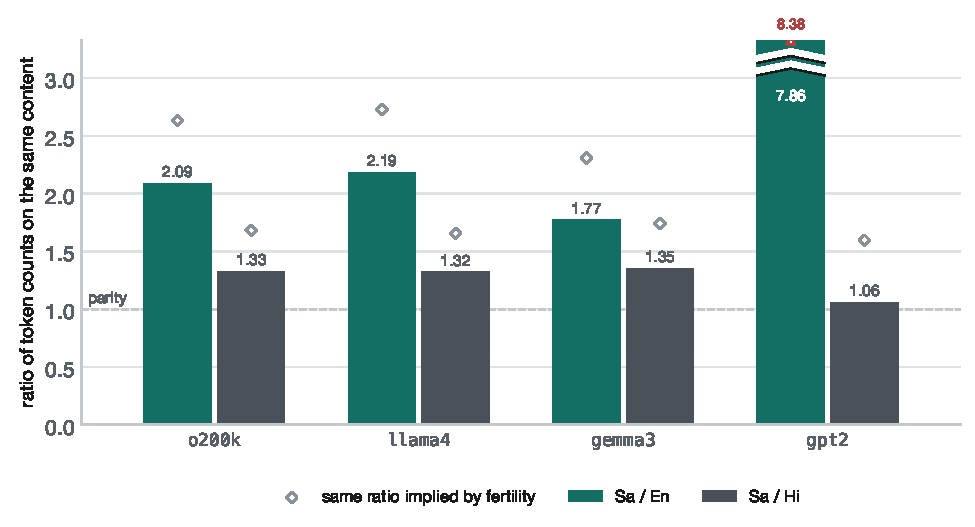
\includegraphics[width=\columnwidth]{figures/parity.pdf}
  \caption{Measured parity (bars) against the ratio fertility implies (diamonds), on
    \numFloresSents{} aligned FLORES-200 devtest sentences, original script. Both series
    are ratios of token counts on the same content; the diamonds are what that ratio would
    have been had it been derived from fertility, and are not themselves a cost per unit
    of content. Every diamond sits above its bar: fertility divides by a Sanskrit word
    count that sandhi and compounding make small, so it overstates the penalty. GPT-2's
    Sanskrit-over-English bar and its diamond run off the axis and carry their values
    instead; the break glyph marks the truncated bar, and the axis is scaled from the
    three arms whose vocabulary size is current practice.}
  \label{fig:parity}
\end{figure}

\begin{table*}[t]
\centering
\footnotesize
\begin{tabular}{lllll}
\toprule
Arm & Vocab. & SLP1 vs \texttt{o200k} & Orig.\ vs \texttt{o200k} & Fert. \\
\midrule
\texttt{T0\_o200k} & 200,019 & 1.835 [1.813, 1.858] & 1.901 [1.874, 1.926] & 3.15 \\
\texttt{T0\_llama4} & 201,135 & 1.882 [1.858, 1.905] & 1.985 [1.958, 2.011] & 3.21 \\
\texttt{T0\_gemma3} & 262,145 & 1.831 [1.809, 1.854] & 1.654 [1.632, 1.675] & 3.13 \\
\texttt{T0\_gpt2} & 50,257 & 2.123 [2.096, 2.151] & 6.562 [6.470, 6.652] & 3.57 \\
\texttt{T3\_sarvam} & 68,096 & 2.416 [2.386, 2.447] & 1.807 [1.782, 1.831] & 4.08 \\
\texttt{T3\_sutra} & 256,061 & 1.930 [1.905, 1.955] & 1.760 [1.735, 1.783] & 3.26 \\
\texttt{T3\_brahmic131k} & 131,072 & 1.873 [1.850, 1.896] & 1.899 [1.872, 1.924] & 3.22 \\
\texttt{T1\_bpe\_raw\_32k}$^{*}$ & 32,000 & \textbf{0.984 [0.970, 0.998]} & n/a & 1.65 \\
\texttt{T1\_bpe\_raw\_64k}$^{*}$ & 64,000 & \textbf{0.887 [0.875, 0.899]} & n/a & 1.49 \\
\texttt{T2\_unigram\_raw\_32k}$^{*}$ & 32,000 & 1.069 [1.055, 1.085] & n/a & 1.80 \\
\texttt{T2\_unigram\_raw\_64k}$^{*}$ & 64,000 & 1.002 [0.988, 1.017] & n/a & 1.69 \\
\bottomrule
\end{tabular}
\caption{Deployed practice on S\=amayik test (prose, primary; $n=2{,}417$ aligned pairs). Tokens per proposition: Sanskrit tokens under the named arm divided by English tokens under a deployed 200k-vocabulary English tokenizer, with 95\% paired bootstrap intervals. This is not a controlled comparison: vocabulary size and training domain vary alongside language, which is what Table~\ref{tab:tppcontrolled} holds fixed. $^{*}$~marks the provisional trained arms. Fertility is in the last column for completeness and is not part of any claim here. Bold marks an interval entirely below 1.0. The second English pivot, and the other three corpora, are in Appendix~\ref{sec:fulltables}. \texttt{T3\_indicsuper} is omitted: no candidate repository resolved.}
\label{tab:tppdeployed}
\end{table*}


\subsection{RQ2 under deployed practice}
\label{sec:rq2-deployed}

Table \ref{tab:tppdeployed} gives tokens per proposition on the primary prose corpus
against the deployed English pivot. Every deployed arm, English-centric and Indic alike,
puts Sanskrit above parity: across prose and FLORES, with the Sanskrit side scored in SLP1
against the deployed \texttt{o200k} pivot, the range is \numDeployedLo--\numDeployedHi{},
with intervals excluding 1.0 throughout. This is the robust finding of the paper. Under
the tokenizers currently shipped, Sanskrit content costs that many times the English
tokens for the same propositions, and the Indic-specialised arms do not fix it.

The trained Sanskrit arms read very differently in the same table. The best of them,
BPE at \numVocabLarge{} pieces, comes in at \numTppBpeSixtyFourDeployed{}
\numTppBpeSixtyFourDeployedCi{}: below parity, with the interval clear of it. Taken at
face value, that is the crossing our design document predicted.

\begin{table*}[t]
\centering
\setlength{\tabcolsep}{4.0pt}
\scriptsize
\begin{tabular}{lllll}
\toprule
Sanskrit arm, over its matched English control & S\=amayik test & S\=amayik test\_ood & Itih\=asa test & FLORES devtest \\
\midrule
\texttt{T1\_bpe\_raw\_32k}$^{*}$ & 1.084 [1.070, 1.098] & 1.086 [1.072, 1.098] & \textbf{0.645 [0.642, 0.649]} & 1.143 [1.131, 1.154] \\
\texttt{T1\_bpe\_raw\_64k}$^{*}$ & 1.035 [1.021, 1.049] & 1.061 [1.048, 1.073] & \textbf{0.598 [0.594, 0.601]} & 1.144 [1.131, 1.155] \\
\texttt{T2\_unigram\_raw\_32k}$^{*}$ & 1.142 [1.128, 1.157] & 1.163 [1.148, 1.176] & \textbf{0.658 [0.655, 0.661]} & 1.206 [1.194, 1.219] \\
\texttt{T2\_unigram\_raw\_64k}$^{*}$ & 1.107 [1.092, 1.121] & 1.156 [1.142, 1.169] & \textbf{0.623 [0.619, 0.626]} & 1.219 [1.206, 1.232] \\
\bottomrule
\end{tabular}
\caption{The controlled comparison. Each row is one matched pair: a trained Sanskrit arm over the English arm sharing its algorithm, its vocabulary size and its training corpus (the two sides of the same S\=amayik and Itih\=asa training splits). The pairs are \texttt{T1\_bpe\_raw\_32k} over \texttt{E1\_bpe\_32k}, \texttt{T1\_bpe\_raw\_64k} over \texttt{E1\_bpe\_64k}, \texttt{T2\_unigram\_raw\_32k} over \texttt{E1\_unigram\_32k}, \texttt{T2\_unigram\_raw\_64k} over \texttt{E1\_unigram\_64k}. Values are tokens per proposition with 95\% paired bootstrap intervals; bold marks an interval entirely below 1.0. Sanskrit is scored in SLP1, English as written, and each arm's name carries its vocabulary size. Pairs: S\=amayik test (prose) 2,417, S\=amayik test\_ood (prose, OOD) 4,047, Itih\=asa test (verse) 11,721, FLORES devtest 1,012. Only the verse corpus stays below parity, and verse carries a meter confound and a 19th-century English translation in the denominator. Both sides of a pair were asked for the same vocabulary size; \texttt{E1\_unigram\_64k} settles on 62,896 pieces, because the EM trainer stops short when the corpus does not support the full vocabulary. That shortfall makes the English side dearer, so it pushes the last row down, against the direction that row is read for.}
\label{tab:tppcontrolled}
\end{table*}


\subsection{RQ2 under the matched control}
\label{sec:rq2-controlled}

It does not survive the control. Table \ref{tab:tppcontrolled} scores the same four
Sanskrit arms against their \texttt{E1} twins, and Figure \ref{fig:denominator} puts the
two readings side by side. On S\=amayik test all \numControlledPairs{} matched pairs sit
above 1.0 with intervals excluding it, from \numTppControlledSamayikLo{}
\numTppControlledBestCi{} to \numTppControlledSamayikHi; the out-of-domain prose split
gives \numTppControlledOodLo--\numTppControlledOodHi{} and FLORES
\numTppControlledFloresLo--\numTppControlledFloresHi, in the same direction and with every
interval above 1.0.

The Sanskrit numerator is the same token count in both ratios, by construction: the same
arm encodes the same sentences. The whole difference between \numTppBpeSixtyFourDeployed{}
and \numTppControlledBest{} is therefore the English denominator, and that much is
arithmetic rather than evidence; the measurement is the size of the change in it. The
control arm spends \numEnTokensEOneBpe{} tokens on the English half of S\=amayik test where
the deployed tokenizer spends \numEnTokensOTwoHundredK, which is
\numEnTokenSavingPct\%{} fewer, because it too was trained on this domain. The apparent
Sanskrit advantage was the English pivot's handicap.

The scope is narrower than the hypothesis it addresses. The only Sanskrit-native
tokenizers here are subword learners trained on raw, sandhied, compounded text, given no
morphological information at all, and our design document lists them as baselines rather
than as the arm it proposes. What is shown is that matched-size raw subword training does
not by itself bring tokens per proposition below English on prose; whether sandhi
splitting or morpheme-constrained merges would is untested here.

Two caveats keep even this provisional. The control equalises domain fit but not corpus
size or diversity, and neither side has seen a monolingual corpus. And one control arm
settles at \numUnigramSixtyFourPieces{} pieces rather than the \numVocabLarge{} requested,
a \numUnigramSixtyFourShortfallPct\%{} shortfall; that makes the English side dearer, so
it pushes its row down rather than up, and the row is above 1.0 regardless.

% TODO(wave1-results): a paragraph reporting the byte-matched control, in which the
% English training text is subsampled to match the Sanskrit side in characters and in
% bytes, and the 128k arms on both sides, with whether the four ratios stay above 1.0.

\begin{figure}[t]
  \centering
  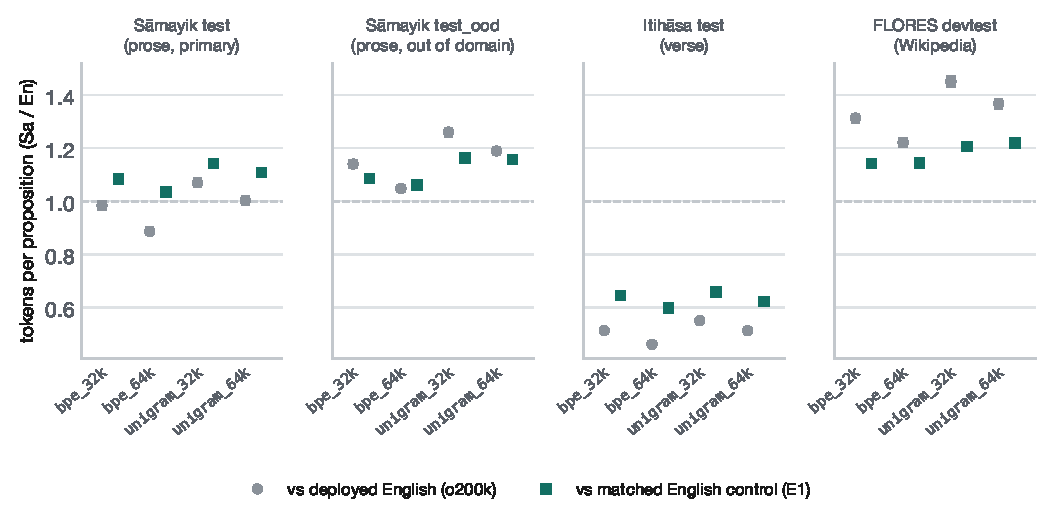
\includegraphics[width=\columnwidth]{figures/denominator.pdf}
  \caption{The same four Sanskrit arms, two English denominators, on each corpus in the
    configured order (prose first). Circles score against the deployed English tokenizer,
    squares against the matched control; the dashed line is parity, and
    \numCiLevel\%{} bootstrap intervals are drawn but are narrower than the markers on
    most points. The in-domain prose panel moves from straddling parity to sitting above it
    when the denominator is controlled; the out-of-domain prose panel sits above parity
    under either denominator. Only the verse panel stays below.}
  \label{fig:denominator}
\end{figure}

\subsection{Verse}
\label{sec:verse}

Itih\=asa is the one corpus where the crossing survives the control:
\numTppControlledItihasaLo--\numTppControlledItihasaHi, every interval excluding 1.0. We
do not read this as a result about tokenization. Itih\=asa is \'sloka, and meter constrains
word choice and rewards compounding; its English side is a nineteenth-century verse
translation whose own verbosity sits in the denominator. Prose was designated primary
before any arm was run, for these reasons; the verse number is a lead, not a finding.

% TODO(wave1-results): a paragraph decomposing the verse ratio into tokens per SLP1
% character on the Sanskrit side and tokens per character on the English side, for Itihasa
% against Samayik, so that the character ratio and the density ratio are separated and the
% crossing can be attributed to one side or the other.

\subsection{Tokens per proposition by sentence length}
\label{sec:length}

A corpus-level ratio compares whole corpora, and the two primary ones differ in length as
well as register: a S\=amayik test pair averages \numSamayikMeanEnWords{} English words to
\numSamayikMeanSaWords{} Sanskrit ones, while over Itih\=asa test the Sanskrit side is
barely longer at \numItihasaMeanSaWords{} against an English side of
\numItihasaMeanEnWords. So the strata ask one question: is the verse result of
Section \ref{sec:verse} a length effect?

They have to be read in pairs, because binning is itself a selection. A sentence's length
on one side is its content plus how wordy that side happened to be, so selecting pairs by a
high English word count selects pairs whose English side is long for their content, and
that side is this ratio's denominator; the ratio then falls as the bin rises whether or not
density changes with length. Binning on the Sanskrit side puts the same selection in the
numerator and makes the ratio rise. Neither stratification is the truth, and together they
bracket it: a gradient keeping its sign under both would be consistent with a length
effect; one that changes sign is selection.

\begin{figure}[!tb]
  \centering
  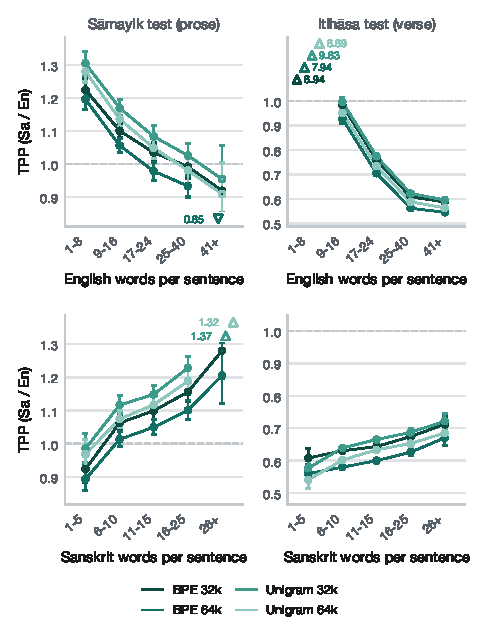
\includegraphics[width=\columnwidth]{figures/length.pdf}
  \caption{Tokens per proposition under the matched control by sentence length, prose left
    and verse right, binned on the English side's word count (top row) and on the
    Sanskrit side's (bottom). Marker shape and hue both identify the matched pair; markers
    are hollow where a bin holds fewer than \numLengthSparseBelow{} pairs, bars are
    \numCiLevel\%{} bootstrap intervals, and the dashed line is parity. Each panel is
    scaled to its own non-sparse bins, so positions are \emph{not} comparable across
    panels and that comparison is numeric, against Table \ref{tab:tppbylength}; a bin whose
    points all run off its panel carries a note instead of a stack of markers. Every
    gradient reverses between the rows, which is what selection on the binned side looks
    like and what a length effect is not.}
  \label{fig:length}
\end{figure}
\begin{table*}[t]
\centering
\setlength{\tabcolsep}{3.5pt}
\scriptsize
\begin{tabular}{lrrrrr}
\toprule
\multicolumn{6}{l}{\emph{(a) Bins cut on the English side}} \\
Matched pair & 1--8 En.\ words & 9--16 En.\ words & 17--24 En.\ words & 25--40 En.\ words & 41+ En.\ words \\
\midrule
\multicolumn{6}{l}{\emph{S\=amayik test (prose)}} \\
$n$ pairs & 835 & 995 & 389 & 187 & 11$^{\dagger}$ \\
BPE 32k & 1.225 [1.191, 1.260] & 1.101 [1.080, 1.122] & 1.035 [1.006, 1.064] & 0.992 [0.957, 1.025] & 0.920 [0.835, 1.006]$^{\dagger}$ \\
BPE 64k & 1.196 [1.165, 1.227] & 1.056 [1.036, 1.077] & 0.979 [0.950, 1.006] & 0.934 [0.900, 0.965] & 0.851 [0.762, 0.940]$^{\dagger}$ \\
Unigram 32k & 1.304 [1.269, 1.339] & 1.170 [1.146, 1.195] & 1.083 [1.052, 1.116] & 1.026 [0.986, 1.061] & 0.955 [0.853, 1.057]$^{\dagger}$ \\
Unigram 64k & 1.280 [1.248, 1.314] & 1.136 [1.113, 1.159] & 1.049 [1.016, 1.079] & 0.981 [0.941, 1.016] & 0.910 [0.818, 1.006]$^{\dagger}$ \\
\midrule
\multicolumn{6}{l}{\emph{Itih\=asa test (verse)}} \\
$n$ pairs & 9$^{\dagger}$ & 419 & 3,945 & 5,658 & 1,690 \\
BPE 32k & $^{\dagger}$ & 0.984 [0.964, 1.002] & 0.760 [0.755, 0.764] & 0.609 [0.605, 0.612] & 0.588 [0.579, 0.598] \\
BPE 64k & $^{\dagger}$ & 0.927 [0.908, 0.946] & 0.705 [0.701, 0.710] & 0.562 [0.559, 0.566] & 0.546 [0.536, 0.555] \\
Unigram 32k & $^{\dagger}$ & 0.996 [0.975, 1.016] & 0.774 [0.769, 0.779] & 0.622 [0.619, 0.626] & 0.596 [0.587, 0.605] \\
Unigram 64k & $^{\dagger}$ & 0.951 [0.933, 0.971] & 0.734 [0.729, 0.739] & 0.589 [0.585, 0.592] & 0.564 [0.555, 0.573] \\
\midrule
\multicolumn{6}{l}{\emph{(b) Bins cut on the Sanskrit side}} \\
Matched pair & 1--5 Sa.\ words & 6--10 Sa.\ words & 11--15 Sa.\ words & 16--25 Sa.\ words & 26+ Sa.\ words \\
\midrule
\multicolumn{6}{l}{\emph{S\=amayik test (prose)}} \\
$n$ pairs & 566 & 973 & 562 & 287 & 29$^{\dagger}$ \\
BPE 32k & 0.924 [0.885, 0.965] & 1.063 [1.039, 1.087] & 1.099 [1.074, 1.125] & 1.156 [1.128, 1.184] & 1.280 [1.196, 1.374]$^{\dagger}$ \\
BPE 64k & 0.894 [0.858, 0.934] & 1.013 [0.991, 1.037] & 1.050 [1.027, 1.074] & 1.101 [1.073, 1.130] & 1.206 [1.123, 1.304]$^{\dagger}$ \\
Unigram 32k & 0.986 [0.944, 1.030] & 1.117 [1.091, 1.144] & 1.148 [1.123, 1.176] & 1.228 [1.195, 1.263] & 1.371 [1.278, 1.492]$^{\dagger}$ \\
Unigram 64k & 0.968 [0.927, 1.013] & 1.075 [1.050, 1.101] & 1.117 [1.093, 1.144] & 1.188 [1.156, 1.222] & 1.319 [1.227, 1.433]$^{\dagger}$ \\
\midrule
\multicolumn{6}{l}{\emph{Itih\=asa test (verse)}} \\
$n$ pairs & 225 & 6,699 & 3,458 & 1,077 & 262 \\
BPE 32k & 0.608 [0.579, 0.638] & 0.630 [0.626, 0.634] & 0.643 [0.637, 0.649] & 0.674 [0.665, 0.685] & 0.712 [0.689, 0.736] \\
BPE 64k & 0.559 [0.534, 0.587] & 0.580 [0.576, 0.584] & 0.600 [0.594, 0.605] & 0.626 [0.617, 0.635] & 0.670 [0.646, 0.695] \\
Unigram 32k & 0.576 [0.549, 0.606] & 0.639 [0.635, 0.643] & 0.665 [0.659, 0.671] & 0.687 [0.678, 0.697] & 0.722 [0.700, 0.745] \\
Unigram 64k & 0.540 [0.514, 0.568] & 0.602 [0.598, 0.606] & 0.633 [0.627, 0.639] & 0.653 [0.643, 0.663] & 0.685 [0.664, 0.708] \\
\bottomrule
\end{tabular}
\caption{Tokens per proposition under the matched control, stratified by sentence length: (a) on the English side's whitespace word count (bin edges 1, 9, 17, 25, 41), (b) on the Sanskrit side's, in the original script (bin edges 1, 6, 11, 16, 26). Cells are the ratio with its 95\% paired bootstrap interval, and nothing is bolded, since which intervals clear 1.0 is read in the prose. Rows are the matched pairs of Table~\ref{tab:tppcontrolled} (BPE 32k is \texttt{T1\_bpe\_raw\_32k} over \texttt{E1\_bpe\_32k}); all four score the same sentences, so the $n$ row belongs to the bin. $^{\dagger}$~marks a bin under 30 pairs; under 10 it stands alone, the ratio left to Table~\ref{tab:tppbylengthall}. The halves are read together: binning on the English side selects pairs whose English side is long for their content, and that side is the denominator, so (a)'s gradient runs down whether or not density changes with length, while in (b) the binned side is the numerator and it runs up. The other two corpora are in Appendix~\ref{sec:lengthstrata}.}
\label{tab:tppbylength}
\end{table*}


Every within-corpus gradient changes sign. Across corpora and matched pairs,
\numLengthGradientsFlipped{} of \numLengthGradientsTotal{} gradients run one way under
English bins and the other under Sanskrit bins (Table \ref{tab:tppbylength},
Figure \ref{fig:length}). On S\=amayik test the controlled ratio
falls from \numLengthEnFirstLo--\numLengthEnFirstHi{} at \numLengthEnFirstBin{} English
words to \numLengthEnLastLo--\numLengthEnLastHi{} at \numLengthEnLastBin, dropping below
1.0 for \numLengthPairsBelowOneEn{} of the \numControlledPairs{} pairs; under Sanskrit bins
the same pairs rise from \numLengthSaFirstLo--\numLengthSaFirstHi{} at
\numLengthSaFirstBin{} Sanskrit words to \numLengthSaLastLo--\numLengthSaLastHi{} at
\numLengthSaLastBin, and the \numLengthPairsBelowOneSa{} pairs below 1.0 are now all in the
\emph{shortest} bin. We therefore draw no claim about tokens per proposition changing with
sentence length from these tables, and in particular the apparent crossing below 1.0 at
long English sentences is not a finding.

The verse and prose separation behaves differently. At every bin where both corpora hold
at least \numLengthSparseBelow{} pairs, verse sits below prose for every matched pair under
\emph{both} stratifications: \numVerseBelowProseComparisons{} of
\numVerseBelowProseTotal{} comparisons, with gaps of \numVerseProseGapMin{} to
\numVerseProseGapMax. That separation is not attributable to length on either side, but it
stays bracketed rather than isolated, since a bin equates the corpora on the side it is cut
on and leaves the other free: at \numEnglishBinExample{} English words Itih\=asa's Sanskrit
side still averages \numEnglishBinItihasaSaWords{} words against S\=amayik's
\numEnglishBinSamayikSaWords, and at \numSanskritBinExample{} Sanskrit words its English
side averages \numSanskritBinItihasaEnWords{} against \numSanskritBinSamayikEnWords.
Nothing here measures meter, and Section \ref{sec:verse}'s confounds stand.

Both counts above are descriptive tallies, not tests: the four matched pairs are near
duplicates and score the same Sanskrit sentences, so neither is that many independent
results, and no multiplicity correction is applied to them or to the intervals read
against 1.0 elsewhere in this paper.

None of it touches Section \ref{sec:rq2-controlled}: the controlled prose result above 1.0
is a statement about the corpus as a whole, and the strata neither strengthen nor weaken
it.

Two diagnostics are reported in the appendix and support no claim here. R\'enyi efficiency
\citep{zouhar-etal-2023-tokenization} was computed for every arm on the primary prose
corpus; it ranks the two trained BPE arms in the opposite order from the controlled ratio
and can be raised without improving the tokenization at all
\citep{cognetta-etal-2024-counterexamples}, so nothing rests on it (Appendix
\ref{sec:renyi}). Appendix \ref{sec:preregistration} sets our predictions against what was
measured, unedited.

\section{Conclusion}
\label{sec:conclusion}

Sanskrit's density is real at the word level and does not survive an English-centric
tokenizer, and matched-size raw subword training does not by itself buy it back on prose.
Length stratification leaves that reading where it stands: the verse and prose separation
survives binning on either side, while every within-corpus gradient reverses with the side
the bins are cut on, which shows selection dominating each stratification and gives no
estimate of a length effect of either sign. The follow-up tests what this leaves open:
sandhi splitting, and morpheme-constrained merges.

% ARR wants Limitations unnumbered, after the conclusion and before the references.
\section*{Limitations}

\paragraph{Verse and meter.} The one corpus on which Sanskrit stays below parity under the
control is verse, where meter is a confound that this design cannot separate from
tokenization. The length strata show that this number is not a sentence-length effect,
under binning on either side, but they do not identify what it is. We report the number and
decline to interpret it.

\paragraph{Translation length bias.} Tokens per proposition divides by a translation on one
side or the other, and a translation is systematically longer than its source
\citep{koppel-ordan-2011-translationese,volansky-etal-2015-features,%
graham-etal-2020-statistical}. The bias is therefore signed, and the signs are not all the
same (Table \ref{tab:direction}). On Itih\=asa the Sanskrit is the source and a
nineteenth-century English verse rendering is the denominator, so the bias runs against the
below-parity reading of Section \ref{sec:verse}, which we decline to make in any case. On
FLORES and on the out-of-domain prose split the English is the source and the Sanskrit the
translation, so the bias sits in the numerator and runs \emph{towards} the above-1.0
conclusion those rows support. On S\=amayik test, the primary corpus for that conclusion,
the direction is mixed by sub-corpus and the sign is unknown; nothing here bounds it, and
we do not claim it is small. FLORES does equalise the two Indic sides, since both are
translations of the same English source, so the Sanskrit-against-Hindi comparison there is
unaffected.

\paragraph{The Indic arms are deployed practice.} The Indic-specialised tokenizers differ
from every other arm in training corpus and vocabulary size. They answer what Sanskrit
costs under current Indic tooling. They cannot answer whether Indic-specialisation helps,
and we do not claim they do.

\paragraph{A single control language.} The control is English, one language, on the
English side of two corpora. Whether the same result holds against a matched Hindi
control, or against a matched control in a third morphologically rich language, is
untested.

\paragraph{No morphology claims.} Nothing here uses gold morpheme boundaries, so this
paper makes no claim about morphological alignment. Measuring whether a tokenizer's
boundaries agree with a language's own \citep{arnett-etal-2025-morphscore} requires a
gold-annotated corpus and is out of scope.

\paragraph{One corpus size.} Every trained arm saw the Sanskrit side, and every control
arm the English side, of the same \numTrainPairsTotal{} training pairs
(S\=amayik \numSamayikTrain, Itih\=asa \numItihasaTrain), after exclusion filtering and
exact deduplication. Tokenizer behaviour changes with corpus scale, and none of these arms
has been trained on a monolingual Sanskrit corpus of realistic size.

% acl.sty anonymises the author block in review mode but does not suppress this section,
% so both the heading and its body are gated on the same switch.
\iffinalmode
\section*{Acknowledgements}

We thank the creators and maintainers of the S\=amayik, Itih\=asa and FLORES-200 corpora
and of the tokenizers evaluated here for releasing them openly. The experimental pipeline,
analyses and manuscript were developed with substantial assistance from AI coding agents
(Claude, Anthropic), operating under the author's direction; all research decisions, the
interpretation of results and the final text are the author's responsibility, and every
number in the paper is regenerated by script from the public results snapshot.
\fi

% Flush every body float before the references, so that no table or figure of the paper is
% deferred into the bibliography.
\FloatBarrier

% acl.sty already issues \bibliographystyle{acl_natbib}; repeating it here puts a second
% \bibstyle into the .aux and BibTeX rejects the file. The style in force is acl_natbib.
\bibliography{refs}

\appendix

\section{Full per-corpus tables}
\label{sec:fulltables}

\begin{table*}[t]
\centering
\scriptsize
\begin{tabular}{llllll}
\toprule
Arm & Vocab. & SLP1 vs \texttt{o200k} & SLP1 vs Llama-4 & Orig.\ vs \texttt{o200k} & Fert. \\
\midrule
\texttt{T0\_o200k} & 200,019 & 1.835 [1.813, 1.858] & 1.802 [1.779, 1.824] & 1.901 [1.874, 1.926] & 3.15 \\
\texttt{T0\_llama4} & 201,135 & 1.882 [1.858, 1.905] & 1.848 [1.825, 1.871] & 1.985 [1.958, 2.011] & 3.21 \\
\texttt{T0\_gemma3} & 262,145 & 1.831 [1.809, 1.854] & 1.798 [1.776, 1.821] & 1.654 [1.632, 1.675] & 3.13 \\
\texttt{T0\_gpt2} & 50,257 & 2.123 [2.096, 2.151] & 2.085 [2.058, 2.113] & 6.562 [6.470, 6.652] & 3.57 \\
\texttt{T3\_sarvam} & 68,096 & 2.416 [2.386, 2.447] & 2.373 [2.342, 2.404] & 1.807 [1.782, 1.831] & 4.08 \\
\texttt{T3\_sutra} & 256,061 & 1.930 [1.905, 1.955] & 1.895 [1.870, 1.921] & 1.760 [1.735, 1.783] & 3.26 \\
\texttt{T3\_brahmic131k} & 131,072 & 1.873 [1.850, 1.896] & 1.839 [1.816, 1.862] & 1.899 [1.872, 1.924] & 3.22 \\
\texttt{T1\_bpe\_raw\_32k}$^{*}$ & 32,000 & \textbf{0.984 [0.970, 0.998]} & \textbf{0.966 [0.952, 0.980]} & n/a & 1.65 \\
\texttt{T1\_bpe\_raw\_64k}$^{*}$ & 64,000 & \textbf{0.887 [0.875, 0.899]} & \textbf{0.871 [0.859, 0.883]} & n/a & 1.49 \\
\texttt{T1\_bpe\_raw\_128k}$^{*}$ & 128,000 & \textbf{0.818 [0.807, 0.830]} & \textbf{0.804 [0.792, 0.815]} & n/a & 1.37 \\
\texttt{T2\_unigram\_raw\_32k}$^{*}$ & 32,000 & 1.069 [1.055, 1.085] & 1.050 [1.036, 1.066] & n/a & 1.80 \\
\texttt{T2\_unigram\_raw\_64k}$^{*}$ & 64,000 & 1.002 [0.988, 1.017] & \textbf{0.984 [0.970, 0.998]} & n/a & 1.69 \\
\texttt{T2\_unigram\_raw\_128k}$^{*}$ & 128,000 & \textbf{0.952 [0.939, 0.966]} & \textbf{0.935 [0.921, 0.949]} & n/a & 1.60 \\
\texttt{T7\_byt5} & 256 & 4.480 [4.424, 4.537] & 4.399 [4.344, 4.458] & 10.816 [10.672, 10.960] & 6.69 \\
\bottomrule
\end{tabular}
\caption{Deployed practice on S\=amayik test (prose), $n=2{,}417$ aligned pairs. Tokens per proposition: Sanskrit tokens under the named arm divided by English tokens under a deployed 200k-vocabulary English tokenizer, with 95\% paired bootstrap intervals. This is not a controlled comparison: vocabulary size and training domain vary alongside language, which is what Table~\ref{tab:tppcontrolled} holds fixed. $^{*}$~marks the provisional trained arms and \texttt{T7\_byt5} the byte-level reference. Fertility is in the last column for completeness and is not part of any claim here. Bold marks an interval entirely below 1.0. \texttt{T3\_indicsuper} is omitted: no candidate repository resolved.}
\label{tab:tppdeployed-samayik-test}
\end{table*}

\begin{table*}[t]
\centering
\scriptsize
\begin{tabular}{llllll}
\toprule
Arm & Vocab. & SLP1 vs \texttt{o200k} & SLP1 vs Llama-4 & Orig.\ vs \texttt{o200k} & Fert. \\
\midrule
\texttt{T0\_o200k} & 200,019 & 1.933 [1.911, 1.954] & 1.905 [1.883, 1.925] & 1.956 [1.933, 1.978] & 3.98 \\
\texttt{T0\_llama4} & 201,135 & 1.985 [1.962, 2.005] & 1.955 [1.933, 1.976] & 2.064 [2.039, 2.087] & 4.04 \\
\texttt{T0\_gemma3} & 262,145 & 1.949 [1.927, 1.970] & 1.920 [1.898, 1.942] & 1.676 [1.655, 1.693] & 3.98 \\
\texttt{T0\_gpt2} & 50,257 & 2.258 [2.231, 2.281] & 2.224 [2.199, 2.248] & 6.986 [6.903, 7.065] & 4.58 \\
\texttt{T3\_sarvam} & 68,096 & 2.556 [2.526, 2.585] & 2.518 [2.489, 2.547] & 1.798 [1.777, 1.818] & 5.17 \\
\texttt{T3\_sutra} & 256,061 & 2.057 [2.033, 2.081] & 2.027 [2.003, 2.049] & 1.827 [1.805, 1.847] & 4.16 \\
\texttt{T3\_brahmic131k} & 131,072 & 1.972 [1.949, 1.993] & 1.943 [1.921, 1.964] & 1.952 [1.929, 1.974] & 4.05 \\
\texttt{T1\_bpe\_raw\_32k}$^{*}$ & 32,000 & 1.139 [1.126, 1.152] & 1.123 [1.109, 1.134] & n/a & 2.31 \\
\texttt{T1\_bpe\_raw\_64k}$^{*}$ & 64,000 & 1.048 [1.036, 1.059] & 1.032 [1.020, 1.044] & n/a & 2.12 \\
\texttt{T1\_bpe\_raw\_128k}$^{*}$ & 128,000 & \textbf{0.977 [0.966, 0.988]} & \textbf{0.963 [0.951, 0.973]} & n/a & 1.98 \\
\texttt{T2\_unigram\_raw\_32k}$^{*}$ & 32,000 & 1.260 [1.244, 1.274] & 1.241 [1.226, 1.255] & n/a & 2.55 \\
\texttt{T2\_unigram\_raw\_64k}$^{*}$ & 64,000 & 1.189 [1.174, 1.202] & 1.171 [1.157, 1.184] & n/a & 2.40 \\
\texttt{T2\_unigram\_raw\_128k}$^{*}$ & 128,000 & 1.115 [1.101, 1.127] & 1.098 [1.085, 1.110] & n/a & 2.26 \\
\texttt{T7\_byt5} & 256 & 4.576 [4.522, 4.627] & 4.508 [4.455, 4.557] & 11.339 [11.206, 11.467] & 8.34 \\
\bottomrule
\end{tabular}
\caption{Deployed practice on S\=amayik test\_ood (prose, OOD), $n=4{,}047$ pairs. Columns as in Table~\ref{tab:tppdeployed-samayik-test}.}
\label{tab:tppdeployed-samayik-test-ood}
\end{table*}

\begin{table*}[t]
\centering
\scriptsize
\begin{tabular}{llllll}
\toprule
Arm & Vocab. & SLP1 vs \texttt{o200k} & SLP1 vs Llama-4 & Orig.\ vs \texttt{o200k} & Fert. \\
\midrule
\texttt{T0\_o200k} & 200,019 & 1.105 [1.100, 1.110] & 1.087 [1.082, 1.092] & 1.152 [1.147, 1.157] & 4.19 \\
\texttt{T0\_llama4} & 201,135 & 1.124 [1.119, 1.129] & 1.105 [1.100, 1.110] & 1.238 [1.232, 1.244] & 4.23 \\
\texttt{T0\_gemma3} & 262,145 & 1.095 [1.090, 1.100] & 1.077 [1.072, 1.082] & 0.996 [0.991, 1.000] & 4.12 \\
\texttt{T0\_gpt2} & 50,257 & 1.249 [1.243, 1.254] & 1.228 [1.223, 1.233] & 4.046 [4.027, 4.064] & 4.67 \\
\texttt{T3\_sarvam} & 68,096 & 1.425 [1.419, 1.432] & 1.402 [1.396, 1.408] & 1.116 [1.111, 1.121] & 5.28 \\
\texttt{T3\_sutra} & 256,061 & 1.169 [1.164, 1.174] & 1.150 [1.145, 1.155] & 1.092 [1.087, 1.097] & 4.33 \\
\texttt{T3\_brahmic131k} & 131,072 & 1.121 [1.115, 1.126] & 1.102 [1.097, 1.107] & 1.151 [1.146, 1.156] & 4.25 \\
\texttt{T1\_bpe\_raw\_32k}$^{*}$ & 32,000 & \textbf{0.513 [0.511, 0.516]} & \textbf{0.505 [0.502, 0.507]} & n/a & 1.90 \\
\texttt{T1\_bpe\_raw\_64k}$^{*}$ & 64,000 & \textbf{0.462 [0.460, 0.464]} & \textbf{0.454 [0.452, 0.457]} & n/a & 1.71 \\
\texttt{T1\_bpe\_raw\_128k}$^{*}$ & 128,000 & \textbf{0.425 [0.423, 0.427]} & \textbf{0.418 [0.416, 0.420]} & n/a & 1.57 \\
\texttt{T2\_unigram\_raw\_32k}$^{*}$ & 32,000 & \textbf{0.551 [0.548, 0.553]} & \textbf{0.542 [0.539, 0.544]} & n/a & 2.04 \\
\texttt{T2\_unigram\_raw\_64k}$^{*}$ & 64,000 & \textbf{0.513 [0.511, 0.516]} & \textbf{0.505 [0.502, 0.507]} & n/a & 1.90 \\
\texttt{T2\_unigram\_raw\_128k}$^{*}$ & 128,000 & \textbf{0.484 [0.481, 0.486]} & \textbf{0.476 [0.473, 0.478]} & n/a & 1.79 \\
\texttt{T7\_byt5} & 256 & 2.549 [2.538, 2.561] & 2.507 [2.496, 2.518] & 6.573 [6.542, 6.602] & 8.54 \\
\bottomrule
\end{tabular}
\caption{Deployed practice on Itih\=asa test (verse), $n=11{,}721$ pairs. Columns as in Table~\ref{tab:tppdeployed-samayik-test}.}
\label{tab:tppdeployed-itihasa-test}
\end{table*}

\begin{table*}[t]
\centering
\scriptsize
\begin{tabular}{llllll}
\toprule
Arm & Vocab. & SLP1 vs \texttt{o200k} & SLP1 vs Llama-4 & Orig.\ vs \texttt{o200k} & Fert. \\
\midrule
\texttt{T0\_o200k} & 200,019 & 2.183 [2.159, 2.207] & 2.169 [2.145, 2.192] & 2.089 [2.066, 2.112] & 3.50 \\
\texttt{T0\_llama4} & 201,135 & 2.256 [2.230, 2.280] & 2.241 [2.216, 2.265] & 2.201 [2.176, 2.225] & 3.56 \\
\texttt{T0\_gemma3} & 262,145 & 2.208 [2.184, 2.230] & 2.194 [2.170, 2.215] & 1.790 [1.769, 1.808] & 3.50 \\
\texttt{T0\_gpt2} & 50,257 & 2.534 [2.502, 2.562] & 2.518 [2.486, 2.544] & 7.907 [7.807, 7.999] & 3.97 \\
\texttt{T3\_sarvam} & 68,096 & 2.899 [2.865, 2.929] & 2.881 [2.847, 2.911] & 1.880 [1.858, 1.901] & 4.58 \\
\texttt{T3\_sutra} & 256,061 & 2.316 [2.288, 2.342] & 2.301 [2.273, 2.327] & 1.863 [1.840, 1.884] & 3.66 \\
\texttt{T3\_brahmic131k} & 131,072 & 2.244 [2.219, 2.269] & 2.230 [2.205, 2.254] & 2.087 [2.064, 2.110] & 3.57 \\
\texttt{T1\_bpe\_raw\_32k}$^{*}$ & 32,000 & 1.312 [1.297, 1.327] & 1.304 [1.288, 1.318] & n/a & 2.07 \\
\texttt{T1\_bpe\_raw\_64k}$^{*}$ & 64,000 & 1.220 [1.204, 1.234] & 1.212 [1.197, 1.226] & n/a & 1.92 \\
\texttt{T1\_bpe\_raw\_128k}$^{*}$ & 128,000 & 1.145 [1.130, 1.158] & 1.137 [1.123, 1.150] & n/a & 1.80 \\
\texttt{T2\_unigram\_raw\_32k}$^{*}$ & 32,000 & 1.450 [1.432, 1.467] & 1.441 [1.423, 1.458] & n/a & 2.29 \\
\texttt{T2\_unigram\_raw\_64k}$^{*}$ & 64,000 & 1.366 [1.349, 1.382] & 1.357 [1.341, 1.373] & n/a & 2.15 \\
\texttt{T2\_unigram\_raw\_128k}$^{*}$ & 128,000 & 1.283 [1.268, 1.298] & 1.275 [1.259, 1.290] & n/a & 2.02 \\
\texttt{T7\_byt5} & 256 & 5.203 [5.142, 5.259] & 5.170 [5.110, 5.226] & 12.906 [12.747, 13.053] & 7.29 \\
\bottomrule
\end{tabular}
\caption{Deployed practice on FLORES devtest, $n=1{,}012$ pairs. Columns as in Table~\ref{tab:tppdeployed-samayik-test}.}
\label{tab:tppdeployed-flores-devtest}
\end{table*}

\begin{table*}[t]
\centering
\footnotesize
\begin{tabular}{lll}
\toprule
Arm & Vocab. & Sa/Hi (original script) \\
\midrule
\texttt{T0\_o200k} & 200,019 & 1.328 [1.315, 1.342] \\
\texttt{T0\_llama4} & 201,135 & 1.325 [1.312, 1.339] \\
\texttt{T0\_gemma3} & 262,145 & 1.353 [1.339, 1.368] \\
\texttt{T0\_gpt2} & 50,257 & 1.060 [1.050, 1.071] \\
\texttt{T3\_sarvam} & 68,096 & 1.405 [1.390, 1.423] \\
\texttt{T3\_sutra} & 256,061 & 1.413 [1.398, 1.429] \\
\texttt{T3\_brahmic131k} & 131,072 & 1.327 [1.314, 1.341] \\
\bottomrule
\end{tabular}
\caption{Sanskrit over Hindi on FLORES devtest, both sides under the same tokenizer, in the original script. The corresponding SLP1 column is computed and stored in the results file but is not printed: SLP1 encodes the Sanskrit phoneme inventory, so Hindi characters outside it inflate the Hindi token count, which sits in this ratio's denominator and mechanically depresses it. Table~\ref{tab:fertcompfull} documents that failure and counts the sentences it affects. The trained arms are excluded by design: the Hindi pivot is defined over the deployed arms only.}
\label{tab:tpphindi}
\end{table*}

\begin{table*}[t]
\centering
\small
\begin{tabular}{lrrrrrrr}
\toprule
Arm & Sa & Hi & En & Sa/En & Sa/Hi & Sa bytes/tok. & En bytes/tok. \\
\midrule
\texttt{T0\_o200k} & 3.75 & 2.23 & 1.42 & 2.63 & 1.68 & 6.18 & 4.92 \\
\texttt{T0\_llama4} & 3.88 & 2.34 & 1.42 & 2.73 & 1.66 & 5.86 & 4.88 \\
\texttt{T0\_gemma3} & 3.11 & 1.79 & 1.35 & 2.31 & 1.74 & 7.21 & 4.87 \\
\texttt{T0\_gpt2} & 12.49 & 7.82 & 1.49 & 8.38 & 1.60 & 1.63 & 4.88 \\
\bottomrule
\end{tabular}
\caption{Fertility (tokens per whitespace word, columns 2--4) on the same sentences, the ratios that fertility implies (columns 5--6), and UTF-8 bytes per token (columns 7--8). Original script throughout. Fertility is reported for comparability with the literature and is not this paper's measure of cost: Sanskrit's denominator is its word count, which sandhi and compounding make small, so columns 5--6 overstate the penalty that Table~\ref{tab:parity} measures. Bytes per token are not comparable across scripts, since Devanagari is three UTF-8 bytes per character. The SLP1 variants of every column are in Table~\ref{tab:fertcompfull}.}
\label{tab:fertcomp}
\end{table*}

\begin{table*}[t]
\centering
\footnotesize
\begin{tabular}{lllrrrr}
\toprule
Arm & Language & Script & Fertility & s.d. & Bytes/tok. & Words \\
\midrule
\texttt{T0\_o200k} & \texttt{san\_Deva} & original & 3.75 & 1.97 & 6.18 & 16,975 \\
\texttt{T0\_o200k} & \texttt{san\_Deva} & slp1 & 3.50 & 1.92 & 2.38 & 16,975 \\
\texttt{T0\_o200k} & \texttt{hin\_Deva} & original & 2.23 & 1.15 & 7.97 & 25,643 \\
\texttt{T0\_o200k} & \texttt{hin\_Deva} & slp1$^{\dagger}$ & 2.56 & 1.29 & 2.31 & 25,643 \\
\texttt{T0\_o200k} & \texttt{eng\_Latn} & original & 1.42 & 0.72 & 4.92 & 21,901 \\
\texttt{T0\_llama4} & \texttt{san\_Deva} & original & 3.88 & 2.05 & 5.86 & 16,975 \\
\texttt{T0\_llama4} & \texttt{san\_Deva} & slp1 & 3.56 & 1.98 & 2.31 & 16,975 \\
\texttt{T0\_llama4} & \texttt{hin\_Deva} & original & 2.34 & 1.18 & 7.55 & 25,643 \\
\texttt{T0\_llama4} & \texttt{hin\_Deva} & slp1$^{\dagger}$ & 2.57 & 1.30 & 2.27 & 25,643 \\
\texttt{T0\_llama4} & \texttt{eng\_Latn} & original & 1.42 & 0.72 & 4.88 & 21,901 \\
\texttt{T0\_gemma3} & \texttt{san\_Deva} & original & 3.11 & 1.67 & 7.21 & 16,975 \\
\texttt{T0\_gemma3} & \texttt{san\_Deva} & slp1 & 3.50 & 1.94 & 2.36 & 16,975 \\
\texttt{T0\_gemma3} & \texttt{hin\_Deva} & original & 1.79 & 0.96 & 9.49 & 25,643 \\
\texttt{T0\_gemma3} & \texttt{hin\_Deva} & slp1$^{\dagger}$ & 2.52 & 1.30 & 2.30 & 25,643 \\
\texttt{T0\_gemma3} & \texttt{eng\_Latn} & original & 1.35 & 0.73 & 4.87 & 21,901 \\
\texttt{T0\_gpt2} & \texttt{san\_Deva} & original & 12.49 & 7.40 & 1.63 & 16,975 \\
\texttt{T0\_gpt2} & \texttt{san\_Deva} & slp1 & 3.97 & 2.23 & 2.05 & 16,975 \\
\texttt{T0\_gpt2} & \texttt{hin\_Deva} & original & 7.82 & 4.18 & 1.68 & 25,643 \\
\texttt{T0\_gpt2} & \texttt{hin\_Deva} & slp1$^{\dagger}$ & 2.85 & 1.49 & 2.02 & 25,643 \\
\texttt{T0\_gpt2} & \texttt{eng\_Latn} & original & 1.49 & 0.81 & 4.88 & 21,901 \\
\bottomrule
\end{tabular}
\caption{Fertility and compression for every arm, language and script variant. $^{\dagger}$~The Hindi SLP1 rows are approximate and should never be quoted as a measurement of Hindi: SLP1 encodes the Sanskrit phoneme inventory, so of the 1,012 Hindi sentences 513 contain a nukta consonant that the transliterator emits as a literal ASCII digit, and 256 of the resulting strings still contain unconverted Devanagari. Both effects inflate the Hindi token count. No parity number in this paper uses an SLP1 Hindi pivot.}
\label{tab:fertcompfull}
\end{table*}


\subsection{Length strata, all corpora}
\label{sec:lengthstrata}

\begin{table*}[t]
\centering
\setlength{\tabcolsep}{3.5pt}
\scriptsize
\begin{tabular}{lrrrrr}
\toprule
Matched pair & 1--8 En.\ words & 9--16 En.\ words & 17--24 En.\ words & 25--40 En.\ words & 41+ En.\ words \\
\midrule
\multicolumn{6}{l}{\emph{S\=amayik test (prose)}} \\
$n$ pairs & 835 & 995 & 389 & 187 & 11$^{\dagger}$ \\
BPE 32k & 1.225 [1.191, 1.260] & 1.101 [1.080, 1.122] & 1.035 [1.006, 1.064] & 0.992 [0.957, 1.025] & 0.920 [0.835, 1.006]$^{\dagger}$ \\
BPE 64k & 1.196 [1.165, 1.227] & 1.056 [1.036, 1.077] & 0.979 [0.950, 1.006] & \textbf{0.934 [0.900, 0.965]} & \textbf{0.851 [0.762, 0.940]}$^{\dagger}$ \\
Unigram 32k & 1.304 [1.269, 1.339] & 1.170 [1.146, 1.195] & 1.083 [1.052, 1.116] & 1.026 [0.986, 1.061] & 0.955 [0.853, 1.057]$^{\dagger}$ \\
Unigram 64k & 1.280 [1.248, 1.314] & 1.136 [1.113, 1.159] & 1.049 [1.016, 1.079] & 0.981 [0.941, 1.016] & 0.910 [0.818, 1.006]$^{\dagger}$ \\
\midrule
\multicolumn{6}{l}{\emph{S\=amayik test\_ood (prose, OOD)}} \\
$n$ pairs & 515 & 1,565 & 1,108 & 704 & 155 \\
BPE 32k & 1.245 [1.181, 1.313] & 1.142 [1.121, 1.164] & 1.103 [1.080, 1.125] & 1.036 [1.009, 1.059] & \textbf{0.951 [0.904, 0.995]} \\
BPE 64k & 1.234 [1.172, 1.298] & 1.118 [1.097, 1.139] & 1.078 [1.054, 1.100] & 1.010 [0.984, 1.033] & \textbf{0.927 [0.882, 0.970]} \\
Unigram 32k & 1.338 [1.272, 1.413] & 1.223 [1.199, 1.247] & 1.180 [1.155, 1.205] & 1.111 [1.083, 1.137] & 1.013 [0.960, 1.063] \\
Unigram 64k & 1.348 [1.283, 1.420] & 1.222 [1.199, 1.246] & 1.174 [1.149, 1.198] & 1.098 [1.069, 1.124] & 1.001 [0.950, 1.049] \\
\midrule
\multicolumn{6}{l}{\emph{Itih\=asa test (verse)}} \\
$n$ pairs & 9$^{\dagger}$ & 419 & 3,945 & 5,658 & 1,690 \\
BPE 32k & 8.944 [3.647, 21.501]$^{\dagger}$ & 0.984 [0.964, 1.002] & \textbf{0.760 [0.755, 0.764]} & \textbf{0.609 [0.605, 0.612]} & \textbf{0.588 [0.579, 0.598]} \\
BPE 64k & 7.944 [3.061, 19.601]$^{\dagger}$ & \textbf{0.927 [0.908, 0.946]} & \textbf{0.705 [0.701, 0.710]} & \textbf{0.562 [0.559, 0.566]} & \textbf{0.546 [0.536, 0.555]} \\
Unigram 32k & 9.833 [4.104, 23.800]$^{\dagger}$ & 0.996 [0.975, 1.016] & \textbf{0.774 [0.769, 0.779]} & \textbf{0.622 [0.619, 0.626]} & \textbf{0.596 [0.587, 0.605]} \\
Unigram 64k & 8.889 [3.350, 22.228]$^{\dagger}$ & \textbf{0.951 [0.933, 0.971]} & \textbf{0.734 [0.729, 0.739]} & \textbf{0.589 [0.585, 0.592]} & \textbf{0.564 [0.555, 0.573]} \\
\midrule
\multicolumn{6}{l}{\emph{FLORES devtest}} \\
$n$ pairs & 8$^{\dagger}$ & 244 & 464 & 280 & 16$^{\dagger}$ \\
BPE 32k & 1.165 [1.000, 1.336]$^{\dagger}$ & 1.155 [1.127, 1.181] & 1.148 [1.132, 1.165] & 1.136 [1.117, 1.155] & 1.091 [1.045, 1.139]$^{\dagger}$ \\
BPE 64k & 1.206 [1.047, 1.375]$^{\dagger}$ & 1.164 [1.136, 1.191] & 1.151 [1.133, 1.170] & 1.130 [1.111, 1.150] & 1.102 [1.057, 1.144]$^{\dagger}$ \\
Unigram 32k & 1.228 [1.086, 1.378]$^{\dagger}$ & 1.212 [1.181, 1.244] & 1.211 [1.191, 1.231] & 1.204 [1.183, 1.226] & 1.143 [1.100, 1.182]$^{\dagger}$ \\
Unigram 64k & 1.286 [1.104, 1.462]$^{\dagger}$ & 1.237 [1.209, 1.266] & 1.227 [1.209, 1.248] & 1.209 [1.188, 1.231] & 1.132 [1.082, 1.179]$^{\dagger}$ \\
\bottomrule
\end{tabular}
\caption{Tokens per proposition under the matched control, stratified by the \textbf{English} side's whitespace word count (bin edges 1, 9, 17, 25, 41). Each cell is the ratio with its 95\% paired bootstrap interval; bold marks an interval entirely below 1.0. Rows name the matched pairs of Table~\ref{tab:tppcontrolled} in short form: BPE 32k is \texttt{T1\_bpe\_raw\_32k} over \texttt{E1\_bpe\_32k}, Unigram 64k is \texttt{T2\_unigram\_raw\_64k} over \texttt{E1\_unigram\_64k}, and so on; all four pairs score the same sentences, so the $n$ row belongs to the bin. $^{\dagger}$~marks a bin with fewer than 30 pairs. Every corpus, at the same bins as the body's Table~\ref{tab:tppbylength}, which carries the two primary ones. Read against its companion on the other side: a gradient that keeps its sign under both stratifications would be consistent with a length effect and one that changes sign is selection, and here all \numLengthGradientsTotal{} change sign.}
\label{tab:tppbylengthall}
\end{table*}

\begin{table*}[t]
\centering
\setlength{\tabcolsep}{3.5pt}
\scriptsize
\begin{tabular}{lrrrrr}
\toprule
Matched pair & 1--5 Sa.\ words & 6--10 Sa.\ words & 11--15 Sa.\ words & 16--25 Sa.\ words & 26+ Sa.\ words \\
\midrule
\multicolumn{6}{l}{\emph{S\=amayik test (prose)}} \\
$n$ pairs & 566 & 973 & 562 & 287 & 29$^{\dagger}$ \\
BPE 32k & \textbf{0.924 [0.885, 0.965]} & 1.063 [1.039, 1.087] & 1.099 [1.074, 1.125] & 1.156 [1.128, 1.184] & 1.280 [1.196, 1.374]$^{\dagger}$ \\
BPE 64k & \textbf{0.894 [0.858, 0.934]} & 1.013 [0.991, 1.037] & 1.050 [1.027, 1.074] & 1.101 [1.073, 1.130] & 1.206 [1.123, 1.304]$^{\dagger}$ \\
Unigram 32k & 0.986 [0.944, 1.030] & 1.117 [1.091, 1.144] & 1.148 [1.123, 1.176] & 1.228 [1.195, 1.263] & 1.371 [1.278, 1.492]$^{\dagger}$ \\
Unigram 64k & 0.968 [0.927, 1.013] & 1.075 [1.050, 1.101] & 1.117 [1.093, 1.144] & 1.188 [1.156, 1.222] & 1.319 [1.227, 1.433]$^{\dagger}$ \\
\midrule
\multicolumn{6}{l}{\emph{S\=amayik test\_ood (prose, OOD)}} \\
$n$ pairs & 571 & 1,500 & 1,046 & 738 & 192 \\
BPE 32k & \textbf{0.769 [0.727, 0.816]} & 0.998 [0.979, 1.018] & 1.101 [1.081, 1.122] & 1.178 [1.151, 1.206] & 1.268 [1.212, 1.326] \\
BPE 64k & \textbf{0.759 [0.717, 0.806]} & \textbf{0.978 [0.959, 0.997]} & 1.076 [1.056, 1.097] & 1.147 [1.122, 1.174] & 1.238 [1.183, 1.295] \\
Unigram 32k & \textbf{0.820 [0.775, 0.870]} & 1.067 [1.044, 1.087] & 1.183 [1.160, 1.208] & 1.260 [1.231, 1.291] & 1.361 [1.301, 1.427] \\
Unigram 64k & \textbf{0.815 [0.770, 0.866]} & 1.065 [1.045, 1.085] & 1.174 [1.153, 1.198] & 1.249 [1.222, 1.279] & 1.349 [1.290, 1.413] \\
\midrule
\multicolumn{6}{l}{\emph{Itih\=asa test (verse)}} \\
$n$ pairs & 225 & 6,699 & 3,458 & 1,077 & 262 \\
BPE 32k & \textbf{0.608 [0.579, 0.638]} & \textbf{0.630 [0.626, 0.634]} & \textbf{0.643 [0.637, 0.649]} & \textbf{0.674 [0.665, 0.685]} & \textbf{0.712 [0.689, 0.736]} \\
BPE 64k & \textbf{0.559 [0.534, 0.587]} & \textbf{0.580 [0.576, 0.584]} & \textbf{0.600 [0.594, 0.605]} & \textbf{0.626 [0.617, 0.635]} & \textbf{0.670 [0.646, 0.695]} \\
Unigram 32k & \textbf{0.576 [0.549, 0.606]} & \textbf{0.639 [0.635, 0.643]} & \textbf{0.665 [0.659, 0.671]} & \textbf{0.687 [0.678, 0.697]} & \textbf{0.722 [0.700, 0.745]} \\
Unigram 64k & \textbf{0.540 [0.514, 0.568]} & \textbf{0.602 [0.598, 0.606]} & \textbf{0.633 [0.627, 0.639]} & \textbf{0.653 [0.643, 0.663]} & \textbf{0.685 [0.664, 0.708]} \\
\midrule
\multicolumn{6}{l}{\emph{FLORES devtest}} \\
$n$ pairs & 5$^{\dagger}$ & 153 & 311 & 457 & 86 \\
BPE 32k & 1.000 [0.868, 1.228]$^{\dagger}$ & 1.073 [1.043, 1.105] & 1.101 [1.082, 1.122] & 1.157 [1.143, 1.172] & 1.223 [1.182, 1.269] \\
BPE 64k & 0.967 [0.864, 1.119]$^{\dagger}$ & 1.075 [1.044, 1.109] & 1.098 [1.078, 1.119] & 1.160 [1.144, 1.175] & 1.225 [1.185, 1.267] \\
Unigram 32k & 1.138 [0.875, 1.398]$^{\dagger}$ & 1.132 [1.098, 1.167] & 1.164 [1.142, 1.188] & 1.221 [1.203, 1.238] & 1.287 [1.242, 1.334] \\
Unigram 64k & 1.095 [0.903, 1.275]$^{\dagger}$ & 1.148 [1.112, 1.187] & 1.172 [1.150, 1.196] & 1.237 [1.218, 1.253] & 1.295 [1.248, 1.346] \\
\bottomrule
\end{tabular}
\caption{Tokens per proposition under the matched control, stratified by the \textbf{Sanskrit} side's whitespace word count in the original script (bin edges 1, 6, 11, 16, 26). Each cell is the ratio with its 95\% paired bootstrap interval; bold marks an interval entirely below 1.0. Rows name the matched pairs of Table~\ref{tab:tppcontrolled} in short form: BPE 32k is \texttt{T1\_bpe\_raw\_32k} over \texttt{E1\_bpe\_32k}, Unigram 64k is \texttt{T2\_unigram\_raw\_64k} over \texttt{E1\_unigram\_64k}, and so on; all four pairs score the same sentences, so the $n$ row belongs to the bin. $^{\dagger}$~marks a bin with fewer than 30 pairs. Every corpus, at the same bins as the body's Table~\ref{tab:tppbylengthsa}, which carries the two primary ones. Read against its companion on the other side: a gradient that keeps its sign under both stratifications would be consistent with a length effect and one that changes sign is selection, and here all \numLengthGradientsTotal{} change sign.}
\label{tab:tppbylengthallsa}
\end{table*}


% TODO(wave1-results): a table of every headline ratio under the block bootstrap beside
% its i.i.d. interval, once the clustered resampling is run.

\section{Arm details}
\label{sec:arms}

\begin{table*}[t]
\centering
\footnotesize
\begin{tabular}{llrl}
\toprule
Arm & Family & Vocab. & What loaded \\
\midrule
\texttt{E1\_bpe\_32k} & E1 & 32,000 & trained here; \texttt{tokenizer.json} sha256 \texttt{f639ee791e50} \\
\texttt{E1\_bpe\_64k} & E1 & 64,000 & trained here; \texttt{tokenizer.json} sha256 \texttt{e57168ce7f9d} \\
\texttt{E1\_unigram\_32k} & E1 & 32,000 & trained here; \texttt{tokenizer.json} sha256 \texttt{62f737185c0c} \\
\texttt{E1\_unigram\_64k} & E1 & 62,896 & trained here; \texttt{tokenizer.json} sha256 \texttt{b21ecf863056} \\
\texttt{T0\_gemma3} & T0 & 262,145 & \texttt{unsloth/gemma-3-4b-it} \\
\texttt{T0\_gpt2} & T0 & 50,257 & \texttt{openai-community/gpt2} \\
\texttt{T0\_llama4} & T0 & 201,135 & \texttt{unsloth/Llama-4-Scout-17B-16E-Instruct} \\
\texttt{T0\_o200k} & T0 & 200,019 & \texttt{o200k\_base} \\
\texttt{T1\_bpe\_raw\_32k}$^{*}$ & T1 & 32,000 & trained here; \texttt{tokenizer.json} sha256 \texttt{e9ae328e26db} \\
\texttt{T1\_bpe\_raw\_64k}$^{*}$ & T1 & 64,000 & trained here; \texttt{tokenizer.json} sha256 \texttt{f74207d923a7} \\
\texttt{T2\_unigram\_raw\_32k}$^{*}$ & T2 & 32,000 & trained here; \texttt{tokenizer.json} sha256 \texttt{09bc885de2ea} \\
\texttt{T2\_unigram\_raw\_64k}$^{*}$ & T2 & 64,000 & trained here; \texttt{tokenizer.json} sha256 \texttt{199e32f30ec1} \\
\texttt{T3\_brahmic131k} & T3 & 131,072 & \texttt{theschoolofai/BrahmicTokenizer-131K} \\
\texttt{T3\_sarvam} & T3 & 68,096 & \texttt{sarvamai/sarvam-1} \\
\texttt{T3\_sutra} & T3 & 256,061 & \texttt{TWO/sutra-mlt256-v2} \\
\bottomrule
\end{tabular}
\caption{Every arm, the identifier that actually loaded, and its id-space size ($\mathrm{len}(\mathrm{tokenizer})$, which counts added special tokens). \texttt{T0\_llama4} and \texttt{T0\_gemma3} load ungated re-uploads of the official releases because the official repositories are gated and the machine running these experiments has no access token; the vocabulary sizes match the published ones, and the mirrors could not be byte-compared against the originals because reading the originals is what the gate prevents. A Hub repository is mutable and these rows carry no revision hash, so the identifier names what was loaded and not which bytes: the load date is the \texttt{timestamp} field of the results file the table is generated from. The sha256 discipline applies only to the arms trained here, whose \texttt{tokenizer.json} this repository holds. Unavailable this run: \texttt{T3\_indicsuper}.}
\label{tab:arms}
\end{table*}


\section{R\'enyi efficiency}
\label{sec:renyi}

R\'enyi efficiency \citep{zouhar-etal-2023-tokenization} scores a tokenizer by how evenly
its token-unigram distribution over a text uses the support that text actually touches, at
$\alpha > 1$ so the head of the distribution weighs more heavily than Shannon entropy
would. We normalise by the observed type count, following the authors' own reference
implementation; the variant normalised by nominal vocabulary size is stored alongside in
the results file. We report it as a diagnostic and nothing more.
\citet{cognetta-etal-2024-counterexamples} construct tokenizers whose R\'enyi efficiency
rises arbitrarily while the tokenization of the text is unchanged or worse, so on its own
the measure supports no claim here.

Table \ref{tab:renyi} reads as follows, at $\alpha = \numRenyiAlpha{}$ on the primary
prose corpus. The deployed arms cluster in a narrow band on Sanskrit,
\numRenyiDeployedLo--\numRenyiDeployedHi, with GPT-2 far below it at \numRenyiGptTwo. The
trained BPE arms sit above that band (\numRenyiBpeThirtyTwo{} at \numVocabSmall{} pieces
and \numRenyiBpeSixtyFour{} at \numVocabLarge) and the trained Unigram arms below it
(\numRenyiUnigramLo--\numRenyiUnigramHi). That comparison crosses columns: the trained
arms are scored in SLP1, which is their only variant, whereas the band just quoted is the
original-script column. The ordering also holds against the deployed arms' own SLP1
column, which runs \numRenyiDeployedSlpOneLo--\numRenyiDeployedSlpOneHi. The English side is lower than the Sanskrit side
for both deployed pivots scored on both halves of the same pairs, and across the pivots
and the matched controls it occupies a band of
\numRenyiEnglishLo--\numRenyiEnglishHi; the two Unigram Sanskrit arms sit at or just
below the foot of that band rather than above it. The reason this section carries no claim is visible in the same
table: R\'enyi ranks the two trained BPE arms in the opposite order from the controlled
tokens per proposition, putting the \numVocabSmall-piece arm above the
\numVocabLarge-piece one (\numRenyiBpeThirtyTwo{} against \numRenyiBpeSixtyFour) where the
controlled ratio prefers \numVocabLarge{} pieces (\numTppControlledBest{} against
\numTppControlledBpeThirtyTwo).

A further caution applies to the Sanskrit-against-English reading in particular.
Normalising by the support the text actually touches makes the measure sensitive to how
many tokens the text contains, and the two sides of the same pairs carry systematically
different token counts, which is this paper's whole finding. The Sanskrit-against-English
comparison in the paragraph above is therefore confounded by token count, and we state it
as an observation about the table rather than as a comparison between the languages.

For the deployed arms the original-script and SLP1 columns are the same text under the
same vocabulary, so the difference between them is what romanisation does to the token
distribution and nothing else. It lowers the measure for every deployed arm but GPT-2, to
\numRenyiDeployedSlpOneLo--\numRenyiDeployedSlpOneHi, and raises GPT-2's from
\numRenyiGptTwo{} to \numRenyiGptTwoSlpOne. We report the direction and do not interpret
it further.

\begin{table*}[t]
\centering
\footnotesize
\begin{tabular}{lrrrr}
\toprule
Arm & orig.\ $\alpha=2.5$ & orig.\ $\alpha=3.0$ & SLP1 $\alpha=2.5$ & SLP1 $\alpha=3.0$ \\
\midrule
\texttt{T0\_o200k} & 0.581 & 0.556 & 0.565 & 0.531 \\
\texttt{T0\_llama4} & 0.575 & 0.549 & 0.560 & 0.527 \\
\texttt{T0\_gemma3} & 0.568 & 0.536 & 0.563 & 0.529 \\
\texttt{T0\_gpt2} & 0.270 & 0.252 & 0.578 & 0.552 \\
\texttt{T3\_sarvam} & 0.570 & 0.541 & 0.556 & 0.530 \\
\texttt{T3\_sutra} & 0.580 & 0.549 & 0.525 & 0.490 \\
\texttt{T3\_brahmic131k} & 0.580 & 0.555 & 0.566 & 0.533 \\
\texttt{T1\_bpe\_raw\_32k}$^{*}$ & n/a & n/a & 0.615 & 0.564 \\
\texttt{T1\_bpe\_raw\_64k}$^{*}$ & n/a & n/a & 0.589 & 0.539 \\
\texttt{T2\_unigram\_raw\_32k}$^{*}$ & n/a & n/a & 0.493 & 0.456 \\
\texttt{T2\_unigram\_raw\_64k}$^{*}$ & n/a & n/a & 0.485 & 0.449 \\
\texttt{T0\_o200k} (English side) & n/a & n/a & 0.490 & 0.461 \\
\texttt{T0\_llama4} (English side) & n/a & n/a & 0.492 & 0.463 \\
\texttt{E1\_bpe\_32k} (English side) & n/a & n/a & 0.507 & 0.468 \\
\texttt{E1\_bpe\_64k} (English side) & n/a & n/a & 0.492 & 0.455 \\
\texttt{E1\_unigram\_32k} (English side) & n/a & n/a & 0.508 & 0.475 \\
\texttt{E1\_unigram\_64k} (English side) & n/a & n/a & 0.500 & 0.466 \\
\bottomrule
\end{tabular}
\caption{R\'enyi efficiency on S\=amayik test (prose), Sanskrit side in both script variants. The English-side rows carry the English text under the named pivot and have no script variant, so their values are placed in the right-hand pair of columns. Reported as a diagnostic only: the measure can be gamed, so it supports no claim in this paper on its own.}
\label{tab:renyi}
\end{table*}


\section{The pre-registration}
\label{sec:preregistration}

\begin{table*}[t]
\centering
\small
\begin{tabular}{p{0.26\textwidth}p{0.42\textwidth}p{0.24\textwidth}}
\toprule
Pre-registered prediction & Measured & Outcome \\
\midrule
T0 fertility on Sanskrit 5--12 & 3.11--3.88 at $\geq$200k vocab; 12.49 for GPT-2 & Refuted, except GPT-2 on Devanagari \\
Hindi 2--4 under the same tokenizer & 1.79--2.34 at $\geq$200k vocab & Held \\
Sa/Hi parity $>1.5$ & 1.060--1.353 & Refuted \\
T3 closes most of the gap vs Hindi & Sa/Hi 1.327--1.413 for T3 against 1.060--1.353 for T0 & Not observed; no gap to close \\
TPP crosses below 1.0 against \texttt{o200k} & 0.887 [0.875, 0.899] on prose; 1.035 [1.021, 1.049] under the matched control & Observed against the pivot, not under control \\
\bottomrule
\end{tabular}
\caption{The pre-registered predictions of the project's design document against what was measured. The predictions were written before any arm was run and are dated in the repository's history. The last row is the paper's central negative result: the crossing is real against the deployed English pivot and disappears against the matched English control, so it is a statement about the pivot's vocabulary and domain rather than about Sanskrit.}
\label{tab:prereg}
\end{table*}


Table \ref{tab:prereg} carries the predictions of our design document, written before any
arm was run, against what was measured. They are reproduced unedited. The first four are
guesses at magnitudes rather than substantive hypotheses, and refuting one's own numeric
guesses is a statement about the guesses. The fifth was written for the sandhi-split,
morpheme-constrained arm this paper does not build, so no outcome is recorded against it;
what its Measured column carries instead is the central negative result for the baselines
this paper does build. The document is dated only by our repository's history and carries
no external timestamp, so it is reported for what it is: a design we did not revise after
seeing the numbers.

\end{document}
